\documentclass[10pt,a4paper,oneside,fleqn]{memoir} 
\usepackage{beamerarticle}
% This file loads some style files
\usepackage{styles/vubhousestyle}  % vub house style: title page, fonts
\usepackage{styles/ulbhousestyle}  % ULB house style: title page, fonts
\usepackage{styles/myListings}     % my source code listings settings
\usepackage{styles/myPackages}     % my packages
\usepackage{styles/myCommands}     % my commands and environments
\usepackage{styles/myDrawingStuff} % my drawing commands 



%%% Specify the content for the VUB title page and title slide

% Important: if you want to remove content from the title page, you have to remove the content from within the curly braces of the relevant command.  For example: if you want to remove the subtitle from the title page,  you have to replace the command \def\vubsubtitle{optional subtitle} by \def\vubsubtitle{}
 
% Pick your type of work:
%\def\vubtypeofwork{Master thesis submitted in order to be awarded the degree of}
\def\vubtypeofwork{Bachelor thesis}
%\def\vubtypeofwork{Masterproef ingediend met het oog op het behalen van de graad van}
%\def\vubtypeofwork{Bachelorproef}
%\def\vubtypeofwork{} % use this to remove it from the title page

% Pick your program:
%\def\vubprogram{Master of Science in Engineering Technology}
\def\vubprogram{Bachelor of Science in Engineering Technology}
%\def\vubprogram{Master of Science in de Industriële Wetenschappen}
%\def\vubprogram{Bachelor of Science in de Industriële Wetenschappen}
%\def\vubprogram{} % use this to remove it from the title page


% Pick your profile:
%\def\vubprofile{Electromechanical Engineering - aeronautics}
%\def\vubprofile{Electromechanical Engineering - mechatronics}
%\def\vubprofile{Electromechanical Engineering - sustainable energy}
%\def\vubprofile{Electromechanical Engineering - transport technology}
%\def\vubprofile{Electronics-ICT - embedded systems}
\def\vubprofile{Electronics-ICT - networks}
%\def\vubprofile{Elektromechanica - duurzame energie}
%\def\vubprofile{Elektromechanica - luchtvaarttechnologie}
%\def\vubprofile{Elektromechanica - mechatronica}
%\def\vubprofile{Elektromechanica - vervoertechnologie}
%\def\vubprofile{Elektronica-ICT - ingebedde systemen}
%\def\vubprofile{Elektronica-ICT - netwerken}
%\def\vubprofile{} % use this to remove it from the title page

\def\vubpretitle{\vubtypeofwork\\ \vubprogram:\\ \vubprofile}
%\def\vubpretitle{} % use this to remove it from the title page

\title{IoT For Sound Pollution} 

\def\vubsubtitle{Sound Level Meter}
%\def\vubsubtitle{} % use this to remove it from the title page

\author{Louka Michaël Grignard} % first name last name

\date{2022-2023}

%\def\vubNDA{Under NDA} % English version
%\def\vubNDA{Onder NDA} % Dutch version
\def\vubNDA{} % use this to remove it from the title page

\def\vubpromoters{promoter: Abdellah Touhafi} % English version
%\def\vubpromoters{promotor: ...} % Dutch version
%\def\vubpromoters{} % use this to remove it from the title page

%\def\vubsupervisors{supervisor: ...} % English version
%\def\vubsupervisors{begeleider: ...} % Dutch version
\def\vubsupervisors{} % use this to remove it from the title page

\def\vubfaculty{ENGINEERING SCIENCES} % English version
%\def\vubfaculty{INGENIEURSWETENSCHAPPEN}  % Dutch version
%\def\vubfaculty{} % use this to remove it from the title page







% \includeonly{chapters/background}

% The second part below is called the DOCUMENT. It contains the source text.
% LaTeX will compile this source text into a typeset document, using the layout rules defined above
\begin{document}  % here content is defined in plain text in a structured way

    %\maketitleVUB % create VUB title page; comment out if not used
    
	\frontmatter % roman page numbers & chapters not numbered
	    %\chapter*{Acknowledgements} 
I thank my promoter and the members of the jury who pointed me in the right direction during the evaluation moments. 

\hfill Louka Grignard

	    %\chapter*{Abstract}\addcontentsline{toc}{chapter}{Abstract}

% \begin{mycomments}
%     An abstract is a summary of the whole thesis and is probably the first part that a reader reads. It should describe the work and set accurate expectations for the reader. It is usually around 200 to 300 words.

%     An abstract in English is required for a master thesis in Engineering Technology. Do not forget to remove this paragraph afterwards.
% \end{mycomments}

This bachelor thesis will cover the process and logic behind the designing of an IoT node able to measure sound. Together with another bachelor thesis, which covers how to build LoRaWAN networks, this research can be used to deploy a sound pollution monitoring network.
Noise pollution is a growing problem in our society. Currently their is insufficient data available to create a good policy to tackle this problem. 

we will give a detailed explanation on why we chose certain components and how these components put constrains on each other. A big part of this thesis will also go over all the theory behind sound and how to measure it. 

Another important part  of this project is the SPI communication protocol which allows the development board to communicate with the ADC. The exact working of this will also be explained in this thesis.

Finally we will discuss how to correctly convert the measured data to values that humans can easily understand. This should help the user to interpret the data correctly and thus create a correct action plan.

% \chapter*{Samenvatting}\addcontentsline{toc}{chapter}{Samenvatting}

% \begin{mycomments}
%     An abstract in Dutch is required for a master thesis in Engineering Technology.
% \end{mycomments}
% \vspace{6cm} % remove this space once the abstract is written
% \textbf{trefwoorden}: \LaTeX, template, TikZ

% \chapter*{Resumé}\addcontentsline{toc}{chapter}{Resumé}


% \begin{mycomments}
%     An abstract in French is required for a master thesis in Engineering Technology.
% \end{mycomments}
% \vspace{6cm} % remove this space once the abstract is written
% \textbf{mots clés}: \LaTeX, template, TikZ

	    %\tableofcontents\newpage
		%\listoffigures\newpage
		%\listoftables\newpage
		%\lstlistoflistings % list of source code listings
		%\chapterOrPart{Nomenclature}\label{sec:nomenclature}

\def\kolomA{1.5cm} \def\kolomB{7cm} \def\kolomC{5.5cm}

% Acronyms
\begin{supertabular}{p{\kolomA}p{\kolomB}}
\multicolumn{2}{l}{\textbf{Acronyms}} \\
\\ 
\acronym{LoRaWAN}{LoRa Wide Area Network}{}
\acronym{IoT}{Internet of Things}{}
\acronym{MAC}{Medium Access Control}{}

\acronym{PCB}{Printed Circuit Board}{}
\acronym{IC}{Integrated Circuit}{}
\acronym{ADC}{Analog-digital-converter}{}
\acronym{DAC}{Digtital-Analog-Converter}{}
\acronym{JFET}{Junction-gate-Field-Effect Transistor}{}
\acronym{LPF}{Low Pass Filter}{}
\acronym{LED}{Light Emmiting Diode}{}
\acronym{RAM}{Random Access Memory}{}

\acronym{DC}{Direct Current}{}
\acronym{AC}{Alternating Current}{}
\acronym{RMS}{Root Mean Squared}{}

\acronym{SPI}{Serial Peripheral Interface}{}
\acronym{CS}{Chip Select}{}
\acronym{SCLK}{Serial Clock}{}
\acronym{MOSI}{Master Out Slave In}{}
\acronym{MISO}{Master In Slave Out}{}
\acronym{SDI}{Slave Device In}{}
\acronym{SDO}{Slave Device Out}{}
\acronym{CPOL}{Clock Polarity}{}
\acronym{CPHA}{Clock Phase}{}
\acronym{DMCLK}{Digital Master Clock}{}
\acronym{AMCLK}{Analog Master Clock}{}
\acronym{CRC}{Cyclic Redundancy Check}{}
\acronym{POR}{Power On Reset}{}
\acronym{OSR}{Over Sampling Ratio}{}

\acronym{DFT}{Discrete Fourier Transform}{}
\acronym{FFT}{Fast Fourier Transform}{}
\acronym{FT}{Fourier Transform}{}

\acronym{SPL}{Sound Pressure Level}{}
\acronym{AOP}{Acoustic Overload Point}{}
\acronym{EIN}{Equivalent Input Noise}{}
\acronym{DNR}{Dynamic Range}{}
\acronym{SNR}{Sound Noise Ratio}{}
\acronym{PSR}{Power Supply Rejection}{}
\acronym{ECM}{Electret Condenser Microphone}{}
\acronym{MEMs}{Micro-Electro-Mechanical systems}{}
\\[+4ex]
\end{supertabular}

% Superscripts
% \begin{supertabular}{p{\kolomA}p{\kolomB}l}
% 	\multicolumn{2}{l}{\textbf{Units}} \\[+2ex]
%     \nomenclature{\texttt{SPL}}{}{Sound Pressure Level}{\texttt{Pa}}
% 	\\[+4ex]
% \end{supertabular}

% Dimensionless numbers
    % \begin{supertabular}{p{\kolomA}p{\kolomB}l} 
    % \multicolumn{2}{l}{\textbf{Dimensionless numbers}} \\[+2ex]
    % \dimensionlessnumber{Ma}{Mach number}{\up{Ma}=\vel/\vel_\up{sound}}
    % \end{supertabular}

% Greek symbols
% \begin{supertabular}{p{\kolomA}p{\kolomB}l}
% 	\multicolumn{2}{l}{\textbf{Greek symbols}} \\[+2ex]
% 	\nomenclature{\alpha}{thermische diffusiviteit}{thermal diffusivity}{m^2/s}
% \\[+4ex]
% \end{supertabular}

% Roman symbols	
% \begin{supertabular}{p{\kolomA}p{\kolomB}l}
% \multicolumn{2}{l}{\textbf{Roman symbols}} \\[+2ex]
% \nomenclature{A}{oppervlak}{area}{m^2}
% \\[+4ex]
% \end{supertabular}


% Subscripts
% \begin{supertabular}{p{\kolomA}p{\kolomB}}
% \multicolumn{2}{l}{\textbf{Subscripts}} \\[+2ex]
% \nomenclaturesubscript{a(tm)}{atmosferisch}{atmospheric} 
% \end{supertabular}

\mode<all> 
% Required because of the \mode* command at the beginning of this file.
% See beameruserfile.pdf section 21.3 for more info


		
	\mainmatter % arabic page numbers & chapters numbered
        \chapter{Literature Review}
\section{LoRa}

\todo{ make a better explanation with images and stuff}

LoRa, which stand for Long Range, is a wireless modulation technique based on the Chirp Spread Spectrum(CSS) technology. It works by sweeping the signal between a lower and an upper frequency over a certain time period, similar to how dolphins and bats communicate. These sweeps are called chirp pulses. 

In order to setup the LoRa modulation you should specify the spreading factor(SF) and the bandwidth. A larger bandwidth will allow for more data to be send but is limited by law. For the sub-gigahertz bands, 915~MHz, 868~MHz and 433~MHz, in europe the bandwidth can be 125~kHz or 250~kHz. In the rest of the world 500~kHz can also be used. LoRa can also be used in the 2.4~GHz band in which case there is an additional option of 1625~kHz. This 2.4~GHz band will allow for higher data rates but will also have a shorter range.

The spreading factor can be between 7 and 12. A higher value will increase resistance to interference and increase the distance over which data can be send but will decrease the data rate. 

One important fact about LoRa is that the on air time is limited by law to 1\%. This means you cannot send for more then 1\% of the time or 36 seconds per hour. This is to prevent the LoRa network from being flooded by a single device. This also means we cannot send large amounts of data over LoRa but rather use it to send small periodic messages. This restriction does not apply to the 2.4~GHz band.

LoRaWAN is a MAC layer protocol which works with LoRa communication. It defines when messages should be send and how they should be formatted. 

\newpage

\section{contiki-ng}

contiki-ng is an open source, cross platform OS for the Internet of Things. There are many implemented standard protocols such as IPv6/6LoWPAN, 6TiSCH, RPL and COAP. It also has a large collection of example applications. This means you can easily create a network of IoT devices and have them communicate with each other. If you want to create your own protocol you can simply look at how the other protocols are implemented and use that as a starting point. This make contiki-ng great in the research world.

In order to run on constrained devices the code footprint is kept low. The OS is on the order of 100~kB while the required RAM can be as low as 10~kB. 

\subsection{Contiki-OS}
\Cite{oikonomouContikiNGOpenSource2022a} goes over how contiki-ng came to be. Below is a short summary of the article.

Contiki-os was developed in 2003 in order to have an OS build for constrained devices. The main strengths of contiki-os were 
\todo{change phrasing of summation for copyright}
\begin{itemize}
    \item Use of the standard C programming language application developers no longer needed to learn a bespoke language such as nesC.
    \item Cooperative multi-threading based API. It greatly simplified application programming, reducing the need for both explicit state machines and locks(compared to event-based API and preemptive thread API, respectively).
    \item Early, standards-compliant support for network protocols such as the Internet Protocol(IP) and IPv6 over Low Power Wireless Personal Area Networks(6LoWPAN) and of the Routing Protocol for Low-Power and Lossy Networks(RPL).
    \item the cooja simulator for IEEE 802.15.4 networks
\end{itemize}

However it still had its limitations. 
\begin{itemize}
    \item Large legacy of old, extremely resource-constrained platforms. The 8-bit and 16-bit low-power microcontrollers which contiki was originally designed for became obsolete over time; 32-bit ARM Cortex-M based devices with more sophisticated low-power mode are the new norm.
    \item Support for non-standard protocols. As the field of wireless sensor network research evolved to become one of the core enabling technologies of the IoT, interoperability and standards became increasingly important. Alongside standardscompliant protocol implementations, the contiki code-base also featured older, experimental, non-standard protocols initially contributed as research artefacts. One such example is the Rime stack.
\end{itemize}

In order to solve these problems contiki required a big overhaul. In order not to break backwards compatibility a new fork was created, contiki-ng. contiki-ng was created with the following goals in mind:
\begin{itemize}
    \item focus on dependable(reliable  and secure) standard-based IPv6 communication
    \item Focus on modern IoT platforms, e.g. ARM Cortex M3 and other 32-bit MCUs
    \item Modernize the structure, configuration, logging and platforms, to reflect the goals above
    \item Improve the documentation, both code API, module description, and tutorials
    \item Implement a more agile development process, with easier inclusion of new features, and with periodic releases.
\end{itemize}

\subsection{OS for this project}
For this project we will be using both contiki-ng and contiki-os. 

contiki-ng will be used to write the final implementation of the RDC layer. This is because contiki-ng is the newer version of contiki-os and is still being actively developed. It also has a larger community and more documentation.

contiki-os will be used as a reference for how to implement the RDC layer. While there are some changes between contiki-os and contiki-ng some things like the network stack are still largely the same. 

\subsection{contiki-ng architecture}
In order to add a RDC layer we first need to understand the contiki-ng architecture.
\begin{itemize}
    \item OS: Platform independent code like kernel, software timers, data structure libraries and networking protocols.
    \item arch: platform specific code to make the OS work on specific hardware. This includes drivers for radio, timers, other on-chip and off-chip peripherals such as UART, SPI, I2C, LED's, buttons and sensors.
    \item examples: 
    \item tests: automated continuous testing
    \item tools: contains utilities such a scripts used to upload firmware, generate documentation, COOJA simulator, etc.
\end{itemize}







\newpage

\section{RDC protocols}

RDC or Radio Duty Cycling protocols are used to reduce the power consumption of a wireless device. They do this by turning off the radio when it is not needed. In theory a radio should only be on when sending a packet or when receiving one. The problem is that we do not know when a packet will be send to us and thus need some kind of logic to allow communication. T

here are 2 groups of RDC protocols, low-power listening and low-power probing. in low-power listening the receiver periodically wakes up and listens to the medium. If the sender wants to send a packet the receiver will stay awake till the packet is received.

in low-power probing, the receiver will periodcally wake up and send out a probe. If the sender wants to send a packet it will be awake and receive this probe. The sender will then send the packet. 

We will now take a more in depth look at the 3 RDC protocols which are implemented in contiki-os.

\todo{give in depth explanation with pictures for the 3 protocols}

\subsection{Low-Power Probing}
The first protocol we will look at is Low-Power Probing or LPP. 

\subsection{X-MAC}

\subsection{contiki-MAC}


One of the protocols that can be used for this is LPP(Low Power Probing). This protocol works by having the receiver wake up periodically and send out a probe. If the sender want to send something, it will be awake and receive this probe. The message can then be send. If the sender is sleeping the probe will be ignored and the receiver will go back to sleep.

The second RDC protocol we will look at is X-MAC. In this protocol the sender will be the one sending out periodic strobes to alert the receiver there is a packet. Once the receiver wakes up it will receive the strobe and send an ACK. The sender will then send the packet. Then both will go back to sleep.
X-MAC has added further optimizations to reduce the power consumption. One of these is that the strobes will contain the receiver address. When a node, which is not the intented receiver, receives the strobe, it will ignore it and go back to sleep. 

finally 

what are RDC protocols

examples: x-mac, lpp 



\section{analasys previous work}

- driver explained


\mode<all> % do not remove


	\appendix % arabic page numbers & chapters lettered
 		%\chapterOrPart{About}\label{ch:about}
This appendix contains a very short description of \LaTeX\ and explains the content and use of this template.

\section{About \LaTeX}\label{sec:aboutlatex}
\LaTeX\ is software to make high-quality technical and scientific documents. It is not a "what you see is what you get" (WYSIWYG) editor such as MS Word or OpenOffice. It is a typesetting engine, which means that it works more like a programming language.

\LaTeX\ requires an input file that contains the source code. The structure of that file is shown below and is discussed in more detail \href{https://en.wikibooks.org/wiki/LaTeX/Document_Structure}{here}.

\begin{verbatim}
    \documentclass[options]{class}
        This part is called the PREAMBLE, here:
        - packages are loaded that enhance the capabilities of LaTeX
        - settings are defined such as: margins, fonts, line spacing, ...
        
    \begin{document}
        This part is called the DOCUMENT, here:
        - content is provided in plain text format
    \end{document}
\end{verbatim}

\subsection{Document class}
The input file starts with the command \textbackslash\verb|documentclass[options]{class}|, where the parameter \texttt{class} stands for the name of a certain class file, recognised by the extension \texttt{.cls}. In a class file the layout standard is defined which tells \LaTeX\ how to format your content. The parameter \texttt{options} customizes the behaviour of the document class by setting parameters such as font size, paper size, etc.

This template uses the class file \texttt{memoir} but many other class files exist such as \texttt{article}, \texttt{report}, \texttt{book},\dots. A comprehensive list of class files can be consulted \href{https://ctan.org/topic/class}{at CTAN}.

\subsection{Preamble}
The next part in the input file is called the \texttt{preamble}. In this part, packages are loaded that enhance the capabilities of \LaTeX. This is typically done in so-called style files with the extension \texttt{.sty}. The packages that are loaded in this template can be found in the style file \texttt{styles/myPackages} and \texttt{styles/myListings}. The use and purpose of some of the loaded packages are discussed further in this chapter. Currently there exist around 4000 packages for \LaTeX\ for all kind of applications. The comprehensive list of all packages can be consulted \href{https://www.ctan.org/pkg/}{at CTAN}.

In the \texttt{preamble} a user can also define his/her own commands and environments. In this template, this is done in the other style files in the folder \texttt{styles}.

\subsection{Entering content}
The actual content of your work is enclosed between the commands \textbackslash\verb|begin{document}| and \textbackslash\verb|end{document}|. When you have a lot of content, you will typically divide it over several files. Files with content have the extension \texttt{.tex}. Content is added as plain text, combined with embedded \LaTeX-commands for specific typeset results. To include files in your input file, you can use the command: \textbackslash\verb|include{filename}| or \textbackslash\verb|input{filename}|.

The command \textbackslash\verb|include{filename}| is used to include chapters. It will process all the floats (figures and tables) from the previous chapter and cause a page break so that the next chapter can start on a new page. It will also start a new auxiliary file in the background to keep track of the locations of figures, tables and equation within the chapter for proper cross-referencing. Inspect the file \texttt{mainReport.tex} to see what chapters are included in this template. 

The command \textbackslash\verb|input{filename}| only imports the content from filename.tex into the target file. It's equivalent to typing all the content from filename.tex into the current file at the location of the \textbackslash\verb|input{filename}| command.

The content is structured for the reader by using commands such as \textbackslash\verb|chapter{name}|,\\ \textbackslash\verb|section{name}|, \textbackslash\verb|subsection{name}|, etc.

More info on how to add content such as text, images, tables and math can be found in \href{https://www.overleaf.com/learn/latex/Learn_LaTeX_in_30_minutes}{Learn \LaTeX\ in 30~minutes}.

\subsection{Compiling your input file}
You have to \texttt{compile} you input file to obtain a typeset PDF document. The processing of your input file is done by a so-called TeX engine. It will parse your input file, line by line, detect the embedded \LaTeX-commands in your input file and act upon them, according the settings  in your class file and packages.

This means that you only have to concentrate on the content, while /LaTeX/ will take care of the formatting!


\section{About this template}
\subsection{Content of the template}
This template will get you started with writing your thesis, report or slides in \href{https://www.latex-project.org}{\LaTeX}. The template contains:
\begin{itemshort}
    \item a title page for VUB and for BRUFACE
    \item acknowledgements
    \item an abstract in English, Dutch and French
    \item a table of contents
    \item a list of figures, tables and listings
    \item a nomenclature
    \item the typical chapters
    \item appendices with useful information on various topics
    \item a bibliography
\end{itemshort}

\subsection{Content of the appendices}
In the appendices you will find useful information about
\begin{itemshort}
    \item \LaTeX\ and this template
    \item formatting of figures, tables, equations and source code
    \item useful \LaTeX\ packages and commands
    \item examples of different types of figures and plots
    \item mathematical and Greek symbols
\end{itemshort}

The template uses the class \href{https://ctan.org/pkg/memoir?lang=en}{memoir}. It is a class for typesetting mathematical works as books, reports and articles.

\subsection{How to start using it}
This template is read-only: this means that you must copy it, before you start using it. A \href{https://vub.cloud.panopto.eu/Panopto/Pages/Sessions/List.aspx?folderID=eb5cbed1-a7f8-4d08-bca3-ad1e00db8d7a}{set of videos} is available that demonstrate the use of this template\footnote{The videos can only be accessed from a VUB-account. Some videos are Dutch spoken, others are English spoken}.

This template can generate a report and slides from the same source code. That's why there are two main files:
\begin{itemize}
    \item \texttt{mainReport.tex}: to compile a report or thesis
    \item \texttt{mainSlides.tex}: to compile the slides
\end{itemize}

Only selected content is put on the slides though. To see all content in this template, you must compile \texttt{mainReport.tex} and/or inspect its source code.

\subsection{How to change the language}

This template is written in English. If you write in another language, you have to adapt the language in three ways (example below is for Dutch):
\begin{enumerate}
    \item Select \texttt{Dutch} as spell check language in Overleaf, via the \texttt{menu} in the upper left corner. Words that do not belong to the selected spell check language will be underlined in red in the editor. 
    \item Select the option \texttt{dutch} in \texttt{styles/myPackages.sty} in these two packages:
    \begin{itemize}
        \item \textbackslash\verb|usepackage[dutch]{babel}|\\
        This will automatically translate standard names:\\
        chapter $\to$ hoofdstuk\\
        table of content $\to$ inhoudsopgave\\
        bibliography $\to$ bibliografie\\\dots
        \item \textbackslash\verb|usepackage[dutch]{cleveref}|\\
        This will automatically translate cross-referencing names:
        \\figure $\to$ figuur\\
        table $\to$ tabel\\
        equation $\to$ vergelijking\\\dots
    \end{itemize}
\end{enumerate}
    

\mode<all> % useful LaTeX packages 
     	%\chapterOrPart{Formatting guidelines}\label{ch:formatting}
Your report or thesis will most probably contain elements such as figures, tables, numbers, units, symbols, mathematical expressions, citations and a bibliography. This chapter contains some guidelines and good practices for the proper formatting of these elements.

\section{Figures}\label{sec:formatfigures}
Figures are visual representations such as drawings, schemes, photos, charts and graphs. Every figure must be referenced in your text, preferably before the figure appears. Some important aspects of a figure are shown in \cref{fig:demofigure} and are discussed below.

\begin{frame}{A figure also requires a clear and well-written caption}
    \begin{figure}\centering
    	    \begin{tikzpicture}[scale=0.8]\node at (0,0) [above right] {\includegraphics[width=0.9\linewidth]{figs/demofigure}};
    			%\draw [help lines] (0,0) grid (14,7); % uncomment to show grid
    			\draw [pin] (8.0,4.0)   |- + (0.5,1) node [right,align=left] {a good-quality figure};
    			\draw [pin] (0.9,1.0)   |- + (0.5,4.7) node [right,align=left] {a numbered identifier under the figure,\\referenced in the text};
    			\draw [pin] ( 2.7,0.6)  -| + (0,   -1) node [below,align=left] {a caption describing: the \textit{what}};
    			\draw [pin] (9.5 ,0.6)  -- + (0,   -1) node [below,align=left] {the \textit{so what}};
    			\draw [pin] (15.3 ,0.6) -- + (0,   -1) node [below,align=left] {the source};
			\end{tikzpicture}
    	\caption{Some important aspects of a figure and its caption}\label{fig:demofigure}
    \end{figure}
\end{frame}

First of all, your figure must be of good quality, which means that careful consideration must be given to graphical excellence and integrity (e.g. resolution, data-ink ratio, lie-factor, legend,\dots). See the excellent work of \textcite{tufte2001} and \textcite{doumont2009} for more information on these topics.

Secondly, your figure must have an unique identifier and a descriptive caption. The identifier is typically the word \textit{Figure} followed by a number. For a short report, these numbers are typically the counting numbers 1, 2, 3, etc. For a thesis or book with different chapters, the numbering of figures restarts at 1 at the beginning of each new chapter, but the chapter number is included in the figure number. See for example the number 4.7 in \cref{fig:demofigure}, which means that this is the seventh figure in chapter 4. The automatic assigning of figure numbers in \LaTeX\ is taken care of by the \verb|\caption| command. If you want the caption to appear under the figure, you must place the \verb|\caption| command on the last line in the figure environment. You can inspect the source code of \cref{fig:demofigure} to verify this.

A descriptive caption is a stand-alone text that must provide enough information to understand the figure, without consulting the text. The first word of the caption should be capitalized. The caption should contain a \textit{what} part and, if possible, a \textit{so what} part. The \textit{what} part clearly explains what is shown on the figure. Try to precise and complete, it's better to have a longer caption than a short incomplete or unclear caption. The \textit{so what} part is a statement and explains what the reader should pay attention to and/or contains a justification for showing the picture.

If you did not make the figure yourself, you must add the reference to the source of the figure at the end of your caption, preceded for instance by the word \verb|source:| If the figure came from an external source but was adapted by you, you can precede the reference to the source by \verb|adapted from:|

\section{Tables}\label{sec:formattables}
Tables are used to present data in a orderly manner. They can contain different kind of elements such as text, numbers and mathematical symbols and expressions. Every table must be referenced in your text, preferably before it appears. Some important aspects of a table are shown in \cref{tab:demotable} and are discussed below.

\begin{table}[htbp]\centering
  	\caption{Some important aspects of a table and its caption}\label{tab:demotable}
    \begin{tikzpicture}[scale=0.8]\node at (0,0) [above right] {\includegraphics[width=0.9\linewidth]{figs/demotable}};
		%\draw [help lines] (0,0) grid (14,7); % uncomment to show grid
		\draw [pin] (0.4,5.8)   |- + (0.5,2)    node [right,align=left] {a numbered identifier above the table,\\referenced in the text};
		\draw [pin] (2.3,4.65)  -| + (-1,0)     node [left,align=left] {a top border};
		\draw [pin] (2.3,4.3)   -| + (-1,-0.6)  node [left,align=left] {column headers};
		\draw [pin] (3,3.9)   -| + (-1.2,-1.5)  node [left,align=left] {some space};
		\draw [pin] (2.3,0.3)   -| + (-1,0)     node [left,align=left] {a bottom border};
		\draw [pin] (2.3,1.5)   -| + (-0.5,0)   node [left,align=left] {a good-quality table};
	    \draw [pin] (2.4,5.8)   |- + (0.5,0.75) node [right,align=left] {a caption describing: the \textit{what}};
		\draw [pin] (11.5,5.8)  |- + (0.5,0.75) node [right,align=left] {the \textit{so what}};
		\draw [pin] (7 ,5.1)    -| + (7.5, -2)  node [below,align=left] {the source};
		\draw [pin] ( 2.8,0.4)  -| + (0,   -1)  node [below,align=left] {column alignment: left};
		\draw [pin] ( 7.8 ,0.4) -- + (0,   -1)  node [below right,align=left] {left};
		\draw [pin] (10.3 ,0.4) -- + (0,   -1)  node [below left,align=right] {right};
		\draw [pin] (10.9 ,0.4) -- + (0,   -1)  node [below right,align=left] {left};
		\draw [pin] (12.1 ,0.4) -- + (0,   -1)  node [below right,align=left] {left};
	\end{tikzpicture}
\end{table}

First of all, your table must be of good quality and should provide clarity on the presented data. This means that careful consideration must be given to graphical excellence and integrity (e.g. readability, data formatting and alignment, data-ink ratio, legend,\dots).

Secondly, your table must have an unique identifier and a descriptive caption. The identifier is typically the word \textit{Table} followed by a number. For a short report, these are typically ordinal numbers such as 1, 2, 3, etc. For a thesis or book with different chapters, the numbering of tables restarts at 1 at the beginning of each new chapter, but the chapter number is included in the table number. Table 3.2 for example refers to the second table in chapter 3. The automatic assigning of table numbers in \LaTeX\ is taken care of by the \verb|\caption| command. If you want the caption to appear above the table, you must place it on the first line in the figure environment. You can inspect the source code of \cref{tab:demotable} to verify this. In Microsoft Word, captions should be added via the \texttt{insert caption} menu command.

A descriptive caption is a stand-alone text that must provide enough information to understand the data in the table, without the need to consult to text. The first word of the caption should be capitalised. The caption should contain a \textit{what} part and, if possible, a \textit{so what} part. The \textit{what} part clearly explains what is shown in the table. Try to precise and complete, it's better to have a longer caption than a short incomplete or unclear caption. The \textit{so what} part is a statement and explains what the reader should pay attention to and/or contains a justification for showing the table.

If you did not obtain the data in the table yourself, you must add the reference to the source of the data at the end of your caption, preceded for instance by the word \verb|source:|

If the table came from an external source but was adapted by you, you can precede the reference to the source by \verb|adapted from:|

\subsection{Column alignment}
The data in the columns should be aligned. Since we read from left to right, it is best to left-align columns (column type \texttt{l} in \LaTeX). This is especially true for text. Columns that contain numbers are an exception. They should be right-aligned (column type \texttt{r}) or aligned at the decimal separator (column type \texttt{S}). This makes it easier to compare numbers in the same column. Columns with symbols and columns with units can be centred (column type \texttt{c}), but they are easier to read when they are left-aligned.

\subsection{Horizontal and vertical lines}
Having too many horizontal and/or vertical lines in a table is considered as visual noise and is distracting to the eye. It also lowers the data-ink ratio. Most of the time, two horizontal lines will do, one at the top of the table (\verb|\toprule| command) and another at the bottom (\verb|\bottomrule| command) as in \cref{tab:demotable}. These lines visually separate the data in the table from the main text. The column headers are separated from the data by some extra space. This separation can also be achieved with a horizontal line (\verb|\midrule| command). Vertical lines are most of the time not required but can be added in some occasions to improve readability.

Compare for instance \cref{tab:demo1} and \cref{tab:demo2}. Both tables contain exactly the same data but \cref{tab:demo2} has the better data-ink ratio and is therefore recommended.

\begin{table}\centering
    \caption{Dummy table with unnecessary horizontal and vertical lines, giving rise to a low data-ink ratio}\label{tab:demo1}
    \begin{tabular}{|l|r|l|l|} 
        \hline
         parameter  &  value & unit         & comment\\[1.5ex]    
         \hline
         voltage    &  12   & \si{\volt}    & given\\
         \hline
         current    &  2    & \si{\ampere}  & given\\
         \hline
        power       &  24   & \si{\watt}    & calculated\\
        \hline
    \end{tabular}
\end{table}

\begin{table}\centering
    \caption{Dummy table with a top and a bottom line only, giving rise to a higher data-ink ratio}\label{tab:demo2}
    \begin{tabular}{lrll}  
        \toprule
         parameter  &  value & unit         & comment\\[1ex]
         voltage    &  12   & \si{\volt}    & given\\
         current    &  2    & \si{\ampere}  & given\\
        power       &  24   & \si{\watt}    & calculated\\
        \bottomrule
    \end{tabular}
\end{table}

\section{Symbols}\label{sec:formatsymbols}
\subsection{Use of symbols}
Symbols are typically used to represent \emph{physical properties} and the units they are expressed in. Physical properties play an important role in physics and engineering. Well-known physical properties are for example the mass, temperature, velocity, pressure and electric current, but there are many others.

Physical quantities can be scalars (e.g. the mass $m$ and temperature $T$) but they can also be vectors (e.g. the force $\vec{F}$ and the velocity $\vec{V}$) or tensors.

The value of a scalar physical quantity is expressed with a number and an associated unit. One can say, for example: the ambient temperature is 298~kelvin. Note that both the name of the physical quantity (ambient temperature) and the name of the unit (kelvin) were written in full. That is perfectly acceptable but not so practical to use in calculations and formulas. That is why we often switch to a compact notation with \emph{symbols}.

For example, one can rewrite the statement regarding the ambient temperature as follows: the ambient temperature $ T_\up{environment}$ is 298~kelvin. Note that we used the symbol $T$ for the temperature. This is merely an agreement and  other symbols for the temperature are also possible. For example, other reference works sometimes use the symbol $\theta$ for the temperature. It is therefore advisable to always consult the symbol list or nomenclature of a scientific publication to find out which symbols were used.

Useful information about the physical quantity can be mentioned in the subscript; in this example the fact that it concerns the temperature of the environment). So $_\up{environment}$ was added as a subscript to the symbol $T$.

There are also symbols for units. For example, the symbol for the kelvin is the uppercase letter K. The above statement concerning the ambient temperature can be rewritten as follows: the ambient temperature $T_\up{environment}$ is \SI{298}{\kelvin}.

\subsection{Formatting of symbols}
One-letter symbols that represent (physical) quantities -- such as for example the temperature $T$ and the voltage $U$ -- are written in italics. Everything else is written upright, as illustrated in the flowchart in \cref{fig:italics}.  Symbols that consist of more than one letter -- such as for instance the Mach number (Ma) or the Net Present Values (NPV) -- are written upright, otherwise they might be mistaken as products. That's why for instance the Reynolds number is written as Re and not as $Re$, because that could be interpreted as the product of the radius $R$ with the eccentricity $e$.

The fact that many symbols must be written upright will give you some kind of struggle, because in the math mode of \LaTeX\, letters are written in italics by default, unless you manually force them upright. The same is true for the Equation editor of Microsoft Word, there too, the standard way of writing is in italics. But no worries, how to deal with this and how to get things right is explained below.

\begin{frame}{Only one-letter symbols that represent quantities are written in italics}
    \begin{figure}\centering
        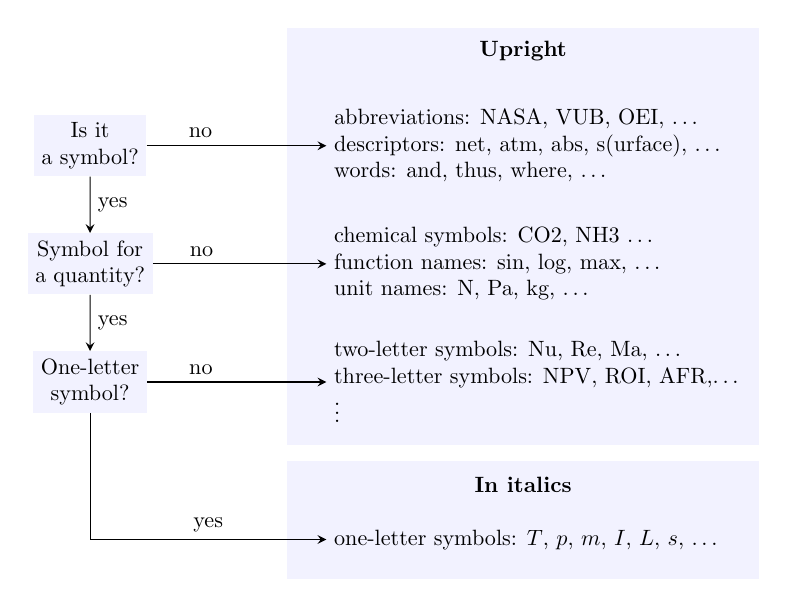
\begin{tikzpicture}[node distance=2cm,every node/.style={scale=0.8}]
            \tikzstyle{examples} = [rectangle, anchor=west,align=left]
            %\tikzstyle{decision} = [rectangle ,align=center,fill=blue!05]
            \tikzstyle{decision} = [rectangle ,align=center,fill=blue!05]
            \tikzstyle{arrow} = [thin,->,>=stealth]
            \tikzstyle{description} = [font=\bfseries]
            \tikzstyle{descriptionbox} = [fill=blue!05,align=left,right]
            %\draw [helpline] (0,0) grid (12,8);
        
            \node (symbol) [decision] at (3,5) {Is it\\ a symbol?};
            \node (quantity) [decision] at (3,3.5) {Symbol for\\ a quantity?};
            \node (oneletter) [decision] at (3,2) {One-letter\\ symbol?};
            
            \fill[descriptionbox] (5.5,1.2) rectangle (11.5,6.5);
            \fill[descriptionbox] (5.5,-0.5) rectangle (11.5,1);
            \node [description] at (8.5,6.2)  {Upright};
            \node [description] at (8.5,0.7)  {In italics};
            
            \node (nosymbol) [examples] at (6,5) {
            abbreviations: NASA, VUB, OEI, \dots\\
            descriptors: net, atm, abs, s(urface), \dots\\
            words: and, thus, where, \dots};
            
            \node (noquantity) [examples] at (6,3.5) {
            chemical symbols: \ch{CO2}, \ch{NH3} \dots\\
            function names: sin, log, max, \dots\\
            unit names: N, Pa, kg, \dots};
            
            \node (nooneletter) [examples] at (6,2) {
            two-letter symbols: Nu, Re, Ma, \dots\\
            three-letter symbols: NPV, ROI, AFR,\dots\\
            $\vdots$};
            
            \node (yesoneletter) [examples] at (6,0) {
            one-letter symbols: $T$, $p$, $m$, $I$, $L$, $s$, \dots};
            
            \draw [arrow] (symbol)   -- node[right] {yes}  (quantity);
            \draw [arrow] (quantity) -- node[right] {yes} (oneletter);
            \draw [arrow] (oneletter) |- node[above,pos=0.75] {yes} (yesoneletter);
            \draw [arrow] (symbol) -- node[above,pos=0.3] {no} (nosymbol);
            \draw [arrow] (quantity) -- node[above,pos=0.28] {no} (noquantity);
            \draw [arrow] (oneletter) -- node[above,pos=0.3] {no} (nooneletter);
        \end{tikzpicture}
        \caption{Flowchart to determine if something must be written upright or in italics: only one-letter symbols for quantities must be written in italics}\label{fig:italics}
    \end{figure}
\end{frame}

Some examples are given below and in \cref{tab:up}. So, as already mentioned, only one-letter symbols for quantities are written in italics:
\begin{align*}
    \text{correct:} \quad & T = \SI{298}{\kelvin} \\
    \text{not correct:} \quad & \up{T} = \SI{298}{\kelvin}
\end{align*}

The same goes for one-letter symbols that appear in subscripts and superscripts. The subscript $p$ for example in the specific heat capacity $c_{p}$ is written in italics because it represents a quantity:
\begin{align*}
    \text{correct:} \quad & c_{p} \quad \text{(because $p$ is a symbol for a quantity)} \\
    \text{not correct:} \quad & c_\up{p} \\
    \text{correct:} \quad & p_\up{gauge} = p_\up{abs} - p_\up{atm}\quad \text{(because the subscripts are not symbols for quantities)} \\
    \text{not correct:} \quad & p_{gauge} = p_{abs} - p_{atm}
\end{align*}

Natural constants are also quantities and their one-letter symbols are therefore also written in italics, as for example, the universal gas constant\footnote{the u in the subscript is written upright because it is not a symbol for a quantity, it's just the first letter of the word 'universal'} $R_\up{u}$ or the speed of light in vacuum $c$. 

\begin{frame}[fragile]{Some stuff is always written upright}\scriptsizebeamer
    \begin{table}\centering
    \caption{Some things are always written upright}\label{tab:up}
        \begin{tabular}{llll}
        \toprule
        type & examples & a \LaTeX\ example & \LaTeX\ result  \\[+1.5ex]
        %\midrule
        descriptions & abs, net, \dots & \verb|$p_\up{atm}$| & $p_\up{atm}$\\
        symbols for units & Pa, kg, \dots & \verb|\si{m^2}| & \si{\square\meter}\\% see package siunitx
        math functions & log, max, \dots & \verb|$\sin\alpha$| & $\sin\alpha$\\
        chemical formulas & \ch{NH3}, \ch{CO2}, \dots & \verb|\ch{CH4}| & $\ch{CH4}$\\ % see package chemformula
        multi-letter symbols & Ma, Nu, \dots & \verb|$\up{Re}=2300$| & $\up{Re}=2300$\\
        acronyms and abbreviations & NPV, NASA, \dots & \verb|$\up{AFR}= 50$| & $\up{AFR}= 50$\\
        \bottomrule
        \end{tabular}
    \end{table}
\end{frame}

More-letter symbols for quantities are written upright:
\begin{align*}
    \text{correct:}     \quad & \up{Ma} = 0.80 \\
    \text{not correct:} \quad & Ma = 0.80 \quad \text{(undesired spacing + looks like $M$ times $a$)}\\
    \text{correct:}     \quad & \text{NPV = 3000~\euro} \\
    \text{not correct:} \quad & NPV = \text{3000~\euro} \quad \text{(undesired spacing + looks like $N$ times $P$ times $V$)}
\end{align*}

Descriptions are written upright:
\begin{align*}
    \text{correct:} \quad & T_\up{environment} = \SI{298}{\kelvin} \\
    \text{not correct:} \quad & T_{environment} = \SI{298}{\kelvin}
\end{align*}

Even if you shorten the descriptive text to make the notation more compact, you still write it upright:
\begin{align*}
    \text{correct:} \quad & T_\up{env} = \SI{298}{\kelvin} \\
    \text{not correct:} \quad & T_{env} = \SI{298}{\kelvin}
\end{align*}

Even descriptions reduced to a single letter are written upright:
\begin{align*}
    \text{correct:} \quad & T_\up{e} = \SI{298}{\kelvin}\quad \text{(because e is not a symbol for a quantity)} \\
    \text{not correct:} \quad & T_{e} = \SI{298}{\kelvin}
\end{align*}

Words are written upright, even when they appear between mathematical expressions:
\begin{align*}
    \text{correct:}     \quad &  U=I R \quad \text{with the current} \quad I=\SI{2}{\ampere}\\
    \text{not correct:} \quad &  U=I R \quad and\ the\ current \quad I=\SI{2}{\ampere}
\end{align*}

Words are written upright, even when they appear in mathematical expressions:
\begin{align*}
    \text{correct:}     \quad &   \eta=\frac{\text{work produced}}{\text{heat received}}\\
    \\
    \text{not correct:} \quad &   \eta=\frac{work\ produced}{heat\ received}
\end{align*}

Symbols for mathematical functions are written upright:
\begin{align*}
    \text{correct:}     \quad &   \sin\alpha\\
    \text{not correct:} \quad &   sin\alpha
\end{align*}

Chemical formulas are written upright:
\begin{align*}
    \text{correct:}     \quad &   \ch{CO2}\\
    \text{not correct:} \quad &       CO_2
\end{align*}

\section{Numbers}\label{sec:formatnumbers}
\subsection{Decimal separator}
In Belgium it is customary to use the comma as the decimal separator (e.g. $\pi\approx$ 3,14), while in the English scientific literature the dot is used ($\pi\approx$ 3.14). 

It is important that you consistently use the same decimal separator throughout your document, otherwise the reader will get confused. If you include figures/tables from English-language literature (that contain numbers with the dot as decimal separator), it is advised to use the dot as the decimal separator for your entire document.

\subsection{Thousands separator}
It is good practise to separate the thousands in a number with a small non-breakable space. This makes a number with many digits easier to read. The \verb|siunitx| package can take care of that, see \cref{sec:siunitx} for more info.

For instance the command \verb|\num{1000000}| produces \num{1000000}. 

The use of the comma as a thousands separator is to be avoided, this to avoid confusion for people in Belgium who are used to the comma as a decimal separator.

\subsection{Significant digits}
It is good practice to write only the significant digits of a number, because a too large number of decimal digits creates a false impression of precision. For instance, a value of 123.456789876~m for a measured length with a simple ruler probably contains decimal digits that are not meaningful. Are you sure up to the level of millimeters, then you can write the number as \SI{123.456}{\meter}. Are you only sure of three significant digits, then you write \SI{123}{\meter}.

If the number of significant digits is lower than the number of digits before the decimal separator, it is better to use a prefix or switch to exponential notation. Are you for example only sure of the first two digits in \SI{123}{\meter}, then you can rewrite it as \SI{0.012}{km} or \SI{1.2E2}{meter}.

\section{Units}\label{sec:formatunits}
Except for dimensionless quantities, numbers without units make no sense. Units are always written upright, never in italics:
\begin{align*}
    \text{correct:} \quad & L = \SI{7}{meter} \\
    \text{not correct:} \quad & L = 7 \; meter
\end{align*}

Symbols for units, like the letter m for meter, are also written upright:
\begin{align*}
    \text{correct:} \quad & L = \SI{7}{\meter} \\
    \text{not correct:} \quad & L = 7 \; m
\end{align*}

In this way there can be no confusion between the symbol $m$ that is used for mass and the symbol m that is used for meter. And so, for example, $A$ represents an area in \si{\square\meter} and the A written upright represents the unit ampere for electric current.

Do not use abbreviations for units. Use the symbol or the full name:
\begin{align*}
    \text{correct:} \quad & \text{s or second; m/s or meters per second} \\
    \text{not correct:} \quad & \text{sec, mps}
\end{align*}

The symbol used for a unit is never written in the plural form:
\begin{align*}
    \text{correct:} \quad & z = \SI{120}{\centi\meter}\\
    \text{not correct:} \quad & z = 120 \; \up{cms}
\end{align*}

No full stop is put after a unit, unless that unit is at the end of a sentence:
\begin{align*}
    \text{correct:} \quad & \text{The length of the tube is 70~cm.}\\
    \text{correct:} \quad & \text{The tube is 70~cm long.} \\
    \text{not correct:} \quad & \text{The tube is 70~cm. long.}
\end{align*}

Prefixes representing a multiplication factor (\cref{t:factors}) are also written upright and written together with the symbol of the unit
\begin{align*}
    \text{correct:} \quad & \pres_\up{1} = \SI{700}{\kilo\pascal} \\
    \text{not correct:} \quad & \pres_\up{1} = 700 \, \up{k \, Pa}
\end{align*}

\begin{table}\centering
\caption{Some standard prefixes in SI units}\label{t:factors}
    \begin{tabular}{llll}
        \toprule
        factor & prefix & factor & prefix \\[+1.5ex]
        \num{E-1}  & deci  &  \num{E1}  & deca \\
        \num{E-2}  & centi &  \num{E2}  & hecto \\
        \num{E-3}  & milli &  \num{E3}  & kilo \\
        \num{E-6}  & micro &  \num{E6}  & mega \\
        \num{E-9}  & nano  &  \num{E9}  & giga \\
        \num{E-12} & pico  &  \num{E12} & terra \\
        \num{E-15} & femto &  \num{E15} & peta \\
        \bottomrule
    \end{tabular}
\end{table}

\subsection{Spaces}
A number must be kept together with its unit. This can be achieved by putting an unbreakable space between the number and the unit. This will 'glue' the unit to the number, so that the number doesn't end up alone at the end of a line with the unit at the start of the next line.

To achieve this in \LaTeX\ you use the tilde \verb|~| in text mode and the \verb|\;| in math mode. So for instance \verb|80~kg| will appear as 80~kg. Or even better, you can use the package \verb|siunitx| that will take care of the proper spacing for you.

In Microsoft Word you must type \textsc{shift-ctrl-space} to produce an unbreakable space.

The unit can also be 'glued' to the number by suppressing the space between them, but this is considered as bad practice.
\begin{align*}
    \text{correct:} \quad & \vol =\SI{3}{\cubic\meter} \\
    \text{bad practice:} \quad & \vol = 3 \up{m ^ 3}
\end{align*}

\section{Mathematical expressions}\label{sec:formatmath}
\subsection{Equations}
It is good practice to number your equations, because it allows to cross-reference them from elsewhere in your text. Automatic numbering can be achieved by using the \texttt{equation} environment, as shown in the first law of thermodynamics for closed systems below
\begin{equation}\label{eq:1stlawclosedsystem}
    \Delta E = Q + W.
\end{equation}

To establish a cross-reference, you must first add a label to the equation environment. You can then use this label in a \verb|\cref{...}| command elsewhere. Inspect the source code of \cref{eq:1stlawclosedsystem} to see how this is done.

There are many other math-environments available in \LaTeX\ that can do more complicated things with equations such as splitting, grouping and aligning. More info is available on the Overleaf help page about \href{https://www.overleaf.com/learn/latex/Aligning_equations_with_amsmath}{aligning equations with amsmath}.

\subsection{Multiplication sign}
To write a multiplication of two variables, leave a small space between them or put a proper multiplication operator between them. In math-mode in \LaTeX, use \verb|\cdot| to produce the center dot $\cdot$ or use \verb|\times| to produce the multiplication sign $\times$.

In Microsoft Word, you can use \verb|\bullet| in the equation editor to produce the center dot $\cdot$.

Other symbols, such as the asterisk *, the letter x and the full stop, should be avoided.
\begin{frame}[fragile]{Some good and bad symbols for multiplying}
    \begin{align*}
    \text{correct:} \quad & U = I\, R \\
    \text{correct:} \quad & U = I\cdot R\\
    \text{correct:} \quad & U = I\times R \\
    \text{not recommended:} \quad & U = I * R \\
    \text{bad practice:} \quad & U = I x R \\
    \text{bad practice:} \quad & U = I.R
    \end{align*}
\end{frame}

\subsection{Punctuation}
Equations are part of the sentence structure, which means
punctuation must be respected. See the example below.

Newton's second law is
\begin{equation}\label{eq:newton}
    \vec{F} = m \cdot \vec{a},
\end{equation}
where $\vec{F}$  is the force,  $m$ the mass and $\vec{a}$ the acceleration.




\section{Using other people's work}\label{sec:formatcites}
In your report or thesis you will probably use information from other sources. If you do so, you have to explain to the reader where this information came from and where this information can be found. This is of great importance for the following three reasons:
\begin{enumerate}
    \item it gives proper credit to the authors or creators of your sources
    \item it allows the reader of your work to look-up and consult the source to learn more about a subject
    \item it avoids that you are being suspected of plagiarism
\end{enumerate}

\subsection{Citing}
Citing is the crediting of author(s) of a source, directly in your text. This is done by putting in-text citations in the body of your text. They are typically placed immediately after the information being cited. In \LaTeX\ we use the package \texttt{BibLaTeX} to take care of the citations, see \cref{sec:biblatex} for more info. There are three commands you should know when citing.

The \verb|\cite| command is used to refer to the work itself, as part of the sentence. For example:

\begin{quotation}
The visual display of quantitative information is discussed in \cite{tufte2001}.
\end{quotation}

The \verb|\textcite| command is used to refer to the author(s) of the work, as part of the sentence.
\begin{quotation}
 \textcite{tufte2001} discusses how quantitative information is visually displayed.
\end{quotation}

The \verb|\parencite| command is used to cite the work when the sentence is already complete. In such a case, the citation is just placed between parentheses at the end of the sentence, but before the full stop!
\begin{quotation}
 Quantitative information is visually displayed in different ways \parencite{tufte2001}.
\end{quotation}

There are many different citation styles, see \cref{tab:cites} with three popular citation styles (author-year, numeric and alphabetic) and the effect on the three cite commands discussed above.

\subsection{Sources}
You should use reliable sources, such as articles from scientific journals. Wikipedia for instance, can certainly be useful as inspiration, and help you understand certain things better, but can't be regarded as primary scientific source material. It's better to consult and use the underlying sources that Wikipedia is citing. So in principle, no reference to Wikipedia should appear in your reference list. But of course exceptions are possible.

\subsection{The bibliography}
The bibliography is a list with all the cited sources in your work. It is typically placed at the very end of your document. It must contain the necessary information to find back the references. Typically: the names of the authors, the title of the work, the publication date, details of the publisher and the book/journal.

In this template, the command \verb|\printbibliography| at the end of the main file produces the bibliography. There are many different styles for a bibliography but we advise you to use one of the standard styles. As was already the case with the citations, the package \texttt{BibLaTeX} will take care of the bibliography. See \cref{sec:biblatex} for more info on this package.

\section{English}\label{sec:formatenglish}
In the European Union, British English is mostly used. American English can also be used, if there are reasons to do so. In any case, you should consistently use one type of spelling throughout your entire document, so American and British spelling cannot be mixed. Some examples of the differences between the British and American spelling are shown in \cref{tab:english}.

\begin{table}[b]\centering
	 \caption{Some examples of words in British and American spelling; in the EU, British English is recommended}\label{tab:english}
        \begin{tabular}{ll}
            \toprule
             British        & American\\[+1.5ex]
             analyse        & analyze\\
             aerofoil       & airfoil\\
             aeroplane      & airplane\\
             behaviour      & behavior\\
             centre         & center\\
             colour         & color\\
             defence        & defense\\
             labelled       & labeled\\
             litre          & liter\\
             metre          & meter\\
             modelling      & modeling\\
             modelled       & modeled\\
             mould          & mold\\
             neighbour      & neighbor\\
             programme      & program\\
             vapour         & vapor\\
             \bottomrule
        \end{tabular}
\end{table}

\mode<all> 
% Required because of the \mode* command at the beginning of this file.
% See beameruserfile.pdf section 21.3 for more info











 % formatting guidelines
		%\chapterOrPart{Useful packages}\label{ch:usefulpackages}
This chapter contains an alphabetic list of some useful packages. All the packages that are mentioned here are included in the style file \verb|styles/myPackages.sty|.

\section{biblatex}\label{sec:biblatex}
This package is used for citing and formatting the bibliography. It is a complete implementation of the bibliographic facilities provided by \LaTeX. BibLaTeX provides several standard citations styles, as for example: \verb|authoryear|, \verb|numeric| and \verb|alphabetic| amongst many other non-standard citation styles that are popular in different journals.

You can inspect the current options that are loaded for the BibLaTeX package in the style file \verb|styles/myPackages.sty|. Some common styles and sorting options are shown in \cref{tab:biblatex}. 

\begin{table}\centering
    \caption{Some examples of style and sorting options in BibLaTeX}\label{tab:biblatex}
        \begin{tabular}{lllll}
        \toprule
        \verb|style|& \verb|sorting| & \verb|\cite| example  & cite number         & order in bibliography  \\[+1.5ex]
        authoryear  & nyt            & Rees, 2017 &                     & by name, year, title \\
        authoryear  & none           & Rees, 2017 &                     & by cite order \\
        numeric     & nyt            & [8]        &  as in bibliography & by name, year, title \\
        numeric     & none           & [1]        &  as order in text   & by cite order  \\
        alphabetic  & nyt            & [Ree17]    &                     & by name, year, title \\
        alphabetic  & none           & [Ree17]    &                     & by cite order  \\
        \bottomrule
        \end{tabular}
\end{table}

\begin{table}\centering
    \caption{Some examples of other cite commands}\label{tab:cites}
        \begin{tabular}{rlllll}
        \toprule
            \verb|style|: 	            &	current	style           &	authoryear	&	numeric	    &	alphabetic	\\[+1.5ex]
            \verb|\cite{Rees2017}| 	    &	\cite{Rees2017}	        &	Rees, 2017	&	[1]	        &	[Ree17]	    \\
            \verb|\textcite{Rees2017}| 	&	\textcite{Rees2017}	    &	Rees (2017)	&	Rees [1]	&	Rees [Ree17]\\
            \verb|\parencite{Rees2017}| &	\parencite{Rees2017}	&	(Rees, 2017)&	[1]	        &	[Ree17]	    \\
            \verb|\citeauthor{Rees2017}|&	\citeauthor{Rees2017}	&	Rees	    &	Rees	    &	Rees	    \\
        \bottomrule
        \end{tabular}
\end{table}

Is is good practice to keep your bibliographic references in a separate file, a so-called bibliographic information file, recognised by the extension \verb|.bib|. In this template, this file can be found here: \verb|bib/myBibliography.bib|.

This file is imported with the command \verb|\addbibresource{bib/myBibliography.bib}| in the style file \verb|styles/myPackages.sty|. 

It is convenient and recommended to use separate software to collect and manage your references. A well-known free tool to manage your references is \href{https://www.mendeley.com/}{Mendeley Reference Manager}. It works well together with \href{https://www.mendeley.com/reference-management/web-importer}{Mendeley Web Importer}. This is a browser extension to import reference material that you are watching in your browser into your Mendeley database.  Other well-known free tools are \href{https://www.zotero.org/}{Zotero} and \href{https://www.jabref.org/}{JabRef}, but there exist many others.

Every reference in the bib file must have a unique identifier, a so-called a \verb|BibTeX key|. You can choose this key yourself. An often-used approach to construct this key is to combine the name of the first author and the year of publishing. You can then refer to a BibTeX key with commands such as \verb|\cite|, \verb|\parencite|, \verb|\textcite| or \verb|\citeauthor|. 

See \cref{tab:cites} for some examples of these cite commands. The second column in this table shows the results for the style that is currently loaded in BibLaTeX. \verb|\cite| is used in sentences where the reference is part of the sentence, and the year is there to identify what is being cited. \verb|\parencite| is used to put the citation between parentheses. It is used when the sentence is already complete, and the citation is being added in support. \verb|\textcite| is used in sentences where the name of the author is part of the sentence, and the year is there to identify what is being cited. With \verb|\citeauthor| only the name of the author is shown without a hyperlink to the reference in the bibliography. 

\textcite{Rees2017} made a good overview of the available commands and options in  \href{https://tug.ctan.org/info/biblatex-cheatsheet/biblatex-cheatsheet.pdf}{this cheat sheet}.

More info at \href{https://ctan.org/pkg/biblatex?lang=en}{CTAN: Package BibLaTeX} and at \href{https://www.overleaf.com/learn/latex/Articles/Getting_started_with_BibLaTeX}{Overleaf: getting started with BibLaTeX}.

\section{cancel}\label{sec:cancel}
With this package you can easily show which terms are canceled in equations. For instance, the command \verb|$\cancel{x}$| will produce $\cancel{x}$ and \verb|$\cancelto{0}{z}$| will produce $\cancelto{0}{z}$.

Both commands are also demonstrated in an equation below.
\begin{frame}{With the package \texttt{cancel}, you can cancel terms in equations}
    \begin{align}
    % the command \intertext is handy to put text between equations in the align environment.
    \intertext{For example, for a stationary \dutch{stilstaand} process:}
    &\Delta E_\CV=\Delta U_\CV + \cancel{\Delta\up{KE}_\CV}\quad +\quad\cancelto{\SI{0}{J}}{\Delta\up{PE}_\CV} \\
    \intertext{and the first law for a closed and stationary system simplifies to}
    &\Delta E_\CV=\Delta U_\CV =Q+W\units{J}.
    \end{align}
\end{frame}

More info at \href{https://ctan.org/pkg/cancel?lang=en}{CTAN: Package cancel}.

\section{chemformula}\label{sec:chemformula}
This package allows you to write chemical formulas in a simple way. Consider for instance the formula $\ch{H2O}$ for water. In the table below you will find some bad and good ways to write it in \LaTeX.

\begin{frame}[fragile]{Some good and bad ways to write a chemical formula}\smallbeamer
% option [fragile] needed when using verbatim on slide with \verb|something|
    \begin{center}
        \begin{tabular}{lll}
        \toprule
        \LaTeX\ command & result & remark \\[+1.5ex]
        \verb|H2O|  & H2O &  not correct, 2 not in subscript \\
        \verb|H_2O| & error & underscore not allowed outside math-mode \\
        \verb|$H_2O$|     & $H_2O$& bad practice to write chemicals in italics\\
        \verb|$\mathrm{H_2O}$|   & $\mathrm{H_2O}$ & correct, but heavy syntax\\
        \verb|\ch{H2O}|   & \ch{H2O} & correct and easy syntax\\
        \bottomrule
        \end{tabular}
    \end{center}
\end{frame}

Writing chemical reactions is also possible. For instance:

\verb|\ch{H2O + CO3^2- <=> OH- + HCO3-}|

produces: \ch{H2O + CO3^2- <=> OH- + HCO3-}

More info at \href{https://ctan.org/pkg/chemformula?lang=EN}{CTAN: Package chemformula}.

\section{cleveref}\label{sec:cleveref}
The \texttt{cleveref} package enhances \LaTeX's cross-referencing features. It automatically formats cross-references depending on what they refer to (chapter, section, table, figure, equation,\dots). The normal procedure in \LaTeX\ is to use the \verb|\ref| command preceded with the type of object that is being referred to. With the \verb|\cref| command, this is no longer necessary because the type of object will be automatically detected. This will make your referring more consistent. In \cref{tab:cref} you will see the difference. For instance in the case of figures, you don't have to explicitly write \verb|fig.| in front of every reference to a figure. For references at the beginning of a sentence, the \verb|\Cref| command must be used. 

\begin{table}\centering
    \caption{Some examples of the use of \texttt{\textbackslash cref} and \texttt{\textbackslash Cref}}\label{tab:cref}
        \begin{tabular}{lll}
        \toprule
        command                         & old syntax with \verb|\ref|           & result \\[+1ex]
        \verb|\cref{ch:conclusions}|    & \verb|chapter~\ref{ch:conclusions}|   & \cref{ch:conclusions} \\
        \verb|\cref{sec:siunitx}|       & \verb|section~\ref{sec:siunitx}|      & \cref{sec:siunitx} \\
        \verb|\cref{fig:psat}|          & \verb|fig.~\ref{fig:psat}|            & \cref{fig:psat} \\
        \verb|\cref{tab:mathsymbols}|   & \verb|table~\ref{tab:mathsymbols}|    & \cref{tab:mathsymbols} \\
        \verb|\cref{eq:newton}|         & \verb|eq.~(\ref{eq:newton})|          & \cref{eq:newton} \\
        \verb|\cref{list:factorial}|    & \verb|listing~(\ref{list:factorial})| & \cref{list:factorial} \\
        \midrule
        %\verb|\Cref| commands          &                                       &  \\[+1.5ex]
        \verb|\Cref{ch:conclusions}|    & \verb|Chapter~\ref{ch:conclusions}|   & \Cref{ch:conclusions} \\
        \verb|\Cref{sec:siunitx}|       & \verb|Section~\ref{sec:siunitx}|      & \Cref{sec:siunitx} \\
        \verb|\Cref{fig:psat}|          & \verb|Figure~\ref{fig:psat}|          & \Cref{fig:psat} \\
        \verb|\Cref{tab:mathsymbols}|   & \verb|Table~\ref{tab:mathsymbols}|    & \Cref{tab:mathsymbols} \\
        \verb|\Cref{eq:newton}|         & \verb|Equation~(\ref{eq:newton})|     & \Cref{eq:newton} \\
        \verb|\Cref{list:factorial}|    & \verb|Listing~(\ref{list:factorial})| & \Cref{list:factorial} \\
        \bottomrule
        \end{tabular}
\end{table}

The format for each cross-reference type (chapter, section, figure, table and equation) can be customised in the style file \verb|myPackages.sty|. 

More info at \href{https://ctan.org/pkg/cleveref}{CTAN: Package cleveref}.

\section{hyperref}\label{sec:hyperref}
With this package you can add hyperlinks in your document. For instance, the command:

\verb|\href{https://canvas.vub.be/}{Canvas learning platform}|

will produce this clickable link: \href{https://canvas.vub.be/}{Canvas learning platform}.

More info can be found in \href{https://ctan.org/pkg/hyperref}{CTAN: Package hyperref}.

\section{Listings}\label{sec:listing}
Sometimes, you want to add source code to your document. Proper typesetting will make your code easier to read. General info about typesetting source code in \LaTeX\ can be found in the \href{https://www.overleaf.com/learn/latex/Code_listing}{Overleaf help pages}. You will read that the package \texttt{Listings} is well suited for this propose. The package provides the \texttt{lstlisting} environment as shown in the "Hello world!" example in \cref{list:hello}. As can be seen in the source code of this example, you can specify the language your code is written in, add a caption and a label for cross-referencing.

Many programming languages can be typeset with this package. The names of the recognised languages can be consulted in \href{https://mirror.lyrahosting.com/CTAN/macros/latex/contrib/listings/listings.pdf}{Tabel 1 in the package documentation}. 

\begin{verbatim}
    \begin{lstlisting}[language=Matlab,label={list:hello},
    caption={Hello world in Matlab}]
        disp('Hello, World!');    
    \end{lstlisting}
\end{verbatim}

The result is shown in \cref{list:hello}.

\begin{lstlisting}[language=Matlab,label={list:hello},caption={Hello world in Matlab}]
    disp('Hello world!');  
\end{lstlisting}

Another example of typesetting of source code, this time in Python, is shown in \cref{list:factorial}. Many typesetting properties (such as: font, font size, indents, colours, \dots) can be specified. The package settings in this template can be consulted and adapted in the style file \texttt{styles/myListings.sty}.

\begin{frame}[fragile]{Listings of code can be easily formatted and displayed}
    \begin{lstlisting}[language=Python, caption={Python code to calculate factorial, adapted from \href{https://www.programiz.com/python-programming/examples/factorial-recursion}{programiz}},label={list:factorial}]
    # Factorial of a number via recursion
    def recur_factorial(n):
       if n == 1:
           return n
       else:
           return n*recur_factorial(n-1)
    
    num = int(input("Enter a number: "))
    if num < 0: # check if the number is negative
       print("Sorry, factorial does not exist for negative numbers")
    elif num == 0: # check if the number is zero
       print("The factorial of 0 is 1")
    else:
       print("The factorial of", num, "is", recur_factorial(num))
    \end{lstlisting}
\end{frame}

It is also possible to import code from a file (that you maybe are still working on) with the command \verb|\lstinputlisting{sourcecode_filename.py}|.

More info at \href{https://ctan.org/pkg/listings?lang=en}{CTAN: Package listings}.

\section{longtable}
With this package you can make tables that are larger than one page and continue to the next page(s).

More info can be found in \href{https://ctan.org/pkg/longtable?lang=en}{CTAN: Package longtable}.

\section{pgfplots}
With this package you can make high-quality plots in normal or logarithmic scaling. They are typically drawn in the \verb|axes| environment and plots are added with the command \verb|\addplot|. See for instance \cref{fig:analyticalfunctions} with some plots of analytical functions and \cref{fig:thermalpower} with a plot of external data from a file. See \href{http://pgfplots.sourceforge.net/gallery.html}{this gallery for many more examples}.

More info can be found in \href{https://ctan.org/pkg/pgfplots?lang=en}{CTAN: Package pgfplots}.

\section{siunitx}\label{sec:siunitx}
This package will neatly and correctly format your numbers and units. You will find some examples of commands and their results in \cref{tab:siunitx}.

\begin{frame}[fragile]{With the package \texttt{siuntix}, you can format numbers and units}\scriptsizebeamer
    \begin{table}\centering
        \caption{Some examples of commands available in \texttt{siunitx}}
           % \begin{tabular}{p{8cm}l}
            \begin{tabular}{ll}
                \toprule
                \LaTeX\ command & result \\[+1ex]
                \verb|\num{3.1E3}| & \num{3.1E3} \\ % to correctly format numbers
                \verb|\numlist{50;70;90}| & \numlist{50;70;90}\\ % list of numbers
                \verb|\SI{50}{\degree}| & \SI{50}{\degree}\\ % to format an angle
                \verb|\SI{31}{\celsius}| & \SI{31}{\celsius}\\ % to format an angle
                \verb|\ang{50;5;33}| & \ang{50;5;33}\\ % to format an angle
                \verb|\SI{9.81}{m/s^2}| & \SI{9.81}{m/s^2} \\ % unit symbols will always produce inclined fraction line in units
                \verb|\SI{9.81}{\meter\per\second\squared}| & \SI{9.81}{\meter\per\second\squared} \\ % unit names will format fraction as specified in style file
                \verb|\SI{9.81}{\meter\per\square\second}| & \SI{9.81}{\meter\per\square\second} \\ % unit names will format fraction as specified in style file
                \verb|\SI{9.81}[per-mode=symbol]{\meter\per\square\second}| & \SI[per-mode=symbol]{9.81}{\meter\per\square\second} \\ % inclined fraction line in units
                \verb|\si{\joule\per\second}| & \si{\joule\per\second} \\ % to format units only
                \verb|\SI{5.0}{\joule\per\second}| & \SI{5.0}{\joule\per\second} \\
                \verb|\si[per-mode=fraction]{\joule\per\second}| & \si{\joule\per\second} \\ % horizontal fraction line in units
                \verb|\si[per-mode=symbol]{\joule\per\second}| & \si[per-mode=symbol]{\joule\per\second} \\ % inclined fraction line in units
                \verb|\si{g_{vapour}\per kg_{dry air}}| & \si{g_{vapour}\per kg_{dry air}}\\
                \verb|\SI{4}{\euro\per\kg}| & \SI{4}{\euro\per\kg} \\
                \verb|\SI{2E-4}{\mol\per\cm\squared\per\second}| & \SI{2E-4}{\mol\per\cm\squared\per\second} \\[+1.5ex]
                \bottomrule
            \end{tabular}\label{tab:siunitx}
    \end{table}
\end{frame}

The package also introduces a column type \texttt{S} to align numbers in tables at the decimal separator. Inspect the source code of \cref{tab:tabledemo} to see the application of these column types. Column \texttt{unit} is centred and uses the command \verb|\si{}| to write the units. The columns indicating the initial end final state are of type \texttt{S}.

\begin{frame}{Formatting numbers and units in tables with \texttt{siunitx}}
    \begin{table}[b]\centering
    	\caption{Example of a property table with type \texttt{S} columns to align numbers at decimal separator}
    			\only<presentation>{\footnotesize}
    	\begin{tabular}{ccScSl} % column types: centre, centre, S, centre, S, left align
    		% column type s for units, column type S for values aligned at decimal separator
                \toprule
                 property & unit            & {initial state}       & process & {end state}         & comment   \\[+1.5ex]
                 $m$      & \si{\kilogram}  &  1.0                  &  $=$    &      1.0            & closed      \\
                 $T$      & \si{\celsius}   &  25.0                 &  $=$    &     25.0            & isotherm    \\
                 $\vol$   & \si{m^3}        &  1.00                 &  $>$    &     0.83            & compression \\
                \bottomrule
    	\end{tabular}\label{tab:tabledemo}
    \end{table}
\end{frame}

More info can be found in \href{https://ctan.org/pkg/siunitx?lang=en}{CTAN: Package siunitx}.


\section{TikZ}\label{sec:tikz}
\verb|TikZ| is a powerful drawing tool inside \LaTeX. Here are useful links to learn \verb|TikZ|
\begin{itemize}
    \item \href{https://www.overleaf.com/learn/latex/TikZ_package}{Overleaf documentation on TikZ}
    \item \href{https://cremeronline.com/LaTeX/minimaltikz.pdf}{A very minimal introduction to TikZ}
    \item \href{https://www.math.uni-leipzig.de/~hellmund/LaTeX/pgf-tut.pdf}{PGF/TikZ - Graphics for \LaTeX} 
    \item \href{http://siam.cs.kuleuven.be/sites/siam.cs.kuleuven.be/files/events/tikz_workshop/tikz_introduction.pdf}{A very short introduction to TikZ} 
    
\end{itemize}

You can for instance make simple inline drawings with the command \verb|tikz{}|. For instance the command

\verb|\tikz{\draw[blue] (0,0) rectangle (3cm,2mm)}|

will draw this blue rectangle \tikz{\fill[blue] (0,0) rectangle (3cm,2mm)}.

More complex drawings are typically made within the \verb|tikzpicture| environment. See \cref{ch:drawing} in this document for some examples. Many more examples can be found on \href{http://www.texample.net/tikz/examples/}{TeXample.net}.

More info can be found in \href{https://ctan.org/pkg/tikz?lang=en}{CTAN: Package TikZ}.

\section{todonotes}\label{sec:todonotes}
With the command \verb|\todo| you can insert notes in your document about things that needs to be
done later. For instance the command \verb|\todo{example of a margin note}| renders to the note in the margin you see in the pdf of this document.
\todo{example of a margin note}

The command \verb|\missingfigure{Search for better picture.}|

will insert a placeholder for a picture you still need to add as shown below.
\missingfigure{Search for better picture.}

The command \verb|\listoftodos| will add a list of all todo's. See last page in this document for such a list.

More info can be found in \href{https://ctan.org/pkg/todonotes?lang=en}{CTAN: Package todonotes}.

\mode<all> 
% Required because of the \mode* command at the beginning of this file.
% See beameruserfile.pdf section 21.3 for more info % useful LaTeX packages 
		%\chapterOrPart{Useful commands}\label{ch:usefulcommands}
This chapter contains an alphabetic list of some useful commands. All the commands that are mentioned here are included in the style file \verb|myCommands.sty|.

\section{Basic commands in \LaTeX}
There are several good sources to learn about commands in \LaTeX. See for instance the list below
\begin{itemize}
    \item \href{https://www.ntg.nl/doc/biemesderfer/ltxcrib.pdf}{\LaTeX\ command summary}
    \item \href{https://wch.github.io/latexsheet/}{\LaTeX\ cheat sheet}
    \item \href{https://en.wikibooks.org/wiki/LaTeX/Command_Glossary}{Wikibook: \LaTeX\ command glossary} 
\end{itemize}

Below we will mention some commands that might be of interest for you.

\section{definecolor}
You can define your own colours. For instance:

\verb|\definecolor{VUBorange}{cmyk}{0.00, .78, 1.00, 0.00}|

will define the colour VUBorange. This colour can now be used in your document, as is done on the title page. For instance, the command 

\verb|\textcolor{VUBorange}{This text is in VUB orange}|

will produce: \textcolor{VUBorange}{This text is in VUB orange}.

\section{ensuremath}
The command \verb|\ensuremath| switches to math-mode, if necessary. It is typically used inside \verb|\newcommand|. For instance, the command \verb|$\psat$| will produce $\psat$ but the command without the dollar-signs \verb|\psat| will produce exactly the same result. This is because the command \verb|\ensuremath| is used inside the definition of \verb|\psat| (you can verify this in the style file \verb|myCommnands.sty|) and that will force a switch to math-mode, if not yet in math-mode. This is very convenient because you are no longer obliged to explicitly activate math-mode with the \$-signs, every time you use such a command when writing.

\section{includeonly}
This command is used to reduce the compilation time of your Overleaf project. There are actually two ways to reduce compilation time:
\begin{enumerate}
    \item Reduce the amount of content in the document part. This can be achieved by disabling \verb|\include{path/filename}| commands. Just put a \% sign at the start of the line. For instance: \%\verb|\chapterOrPart{Useful packages}\label{ch:usefulpackages}
This chapter contains an alphabetic list of some useful packages. All the packages that are mentioned here are included in the style file \verb|styles/myPackages.sty|.

\section{biblatex}\label{sec:biblatex}
This package is used for citing and formatting the bibliography. It is a complete implementation of the bibliographic facilities provided by \LaTeX. BibLaTeX provides several standard citations styles, as for example: \verb|authoryear|, \verb|numeric| and \verb|alphabetic| amongst many other non-standard citation styles that are popular in different journals.

You can inspect the current options that are loaded for the BibLaTeX package in the style file \verb|styles/myPackages.sty|. Some common styles and sorting options are shown in \cref{tab:biblatex}. 

\begin{table}\centering
    \caption{Some examples of style and sorting options in BibLaTeX}\label{tab:biblatex}
        \begin{tabular}{lllll}
        \toprule
        \verb|style|& \verb|sorting| & \verb|\cite| example  & cite number         & order in bibliography  \\[+1.5ex]
        authoryear  & nyt            & Rees, 2017 &                     & by name, year, title \\
        authoryear  & none           & Rees, 2017 &                     & by cite order \\
        numeric     & nyt            & [8]        &  as in bibliography & by name, year, title \\
        numeric     & none           & [1]        &  as order in text   & by cite order  \\
        alphabetic  & nyt            & [Ree17]    &                     & by name, year, title \\
        alphabetic  & none           & [Ree17]    &                     & by cite order  \\
        \bottomrule
        \end{tabular}
\end{table}

\begin{table}\centering
    \caption{Some examples of other cite commands}\label{tab:cites}
        \begin{tabular}{rlllll}
        \toprule
            \verb|style|: 	            &	current	style           &	authoryear	&	numeric	    &	alphabetic	\\[+1.5ex]
            \verb|\cite{Rees2017}| 	    &	\cite{Rees2017}	        &	Rees, 2017	&	[1]	        &	[Ree17]	    \\
            \verb|\textcite{Rees2017}| 	&	\textcite{Rees2017}	    &	Rees (2017)	&	Rees [1]	&	Rees [Ree17]\\
            \verb|\parencite{Rees2017}| &	\parencite{Rees2017}	&	(Rees, 2017)&	[1]	        &	[Ree17]	    \\
            \verb|\citeauthor{Rees2017}|&	\citeauthor{Rees2017}	&	Rees	    &	Rees	    &	Rees	    \\
        \bottomrule
        \end{tabular}
\end{table}

Is is good practice to keep your bibliographic references in a separate file, a so-called bibliographic information file, recognised by the extension \verb|.bib|. In this template, this file can be found here: \verb|bib/myBibliography.bib|.

This file is imported with the command \verb|\addbibresource{bib/myBibliography.bib}| in the style file \verb|styles/myPackages.sty|. 

It is convenient and recommended to use separate software to collect and manage your references. A well-known free tool to manage your references is \href{https://www.mendeley.com/}{Mendeley Reference Manager}. It works well together with \href{https://www.mendeley.com/reference-management/web-importer}{Mendeley Web Importer}. This is a browser extension to import reference material that you are watching in your browser into your Mendeley database.  Other well-known free tools are \href{https://www.zotero.org/}{Zotero} and \href{https://www.jabref.org/}{JabRef}, but there exist many others.

Every reference in the bib file must have a unique identifier, a so-called a \verb|BibTeX key|. You can choose this key yourself. An often-used approach to construct this key is to combine the name of the first author and the year of publishing. You can then refer to a BibTeX key with commands such as \verb|\cite|, \verb|\parencite|, \verb|\textcite| or \verb|\citeauthor|. 

See \cref{tab:cites} for some examples of these cite commands. The second column in this table shows the results for the style that is currently loaded in BibLaTeX. \verb|\cite| is used in sentences where the reference is part of the sentence, and the year is there to identify what is being cited. \verb|\parencite| is used to put the citation between parentheses. It is used when the sentence is already complete, and the citation is being added in support. \verb|\textcite| is used in sentences where the name of the author is part of the sentence, and the year is there to identify what is being cited. With \verb|\citeauthor| only the name of the author is shown without a hyperlink to the reference in the bibliography. 

\textcite{Rees2017} made a good overview of the available commands and options in  \href{https://tug.ctan.org/info/biblatex-cheatsheet/biblatex-cheatsheet.pdf}{this cheat sheet}.

More info at \href{https://ctan.org/pkg/biblatex?lang=en}{CTAN: Package BibLaTeX} and at \href{https://www.overleaf.com/learn/latex/Articles/Getting_started_with_BibLaTeX}{Overleaf: getting started with BibLaTeX}.

\section{cancel}\label{sec:cancel}
With this package you can easily show which terms are canceled in equations. For instance, the command \verb|$\cancel{x}$| will produce $\cancel{x}$ and \verb|$\cancelto{0}{z}$| will produce $\cancelto{0}{z}$.

Both commands are also demonstrated in an equation below.
\begin{frame}{With the package \texttt{cancel}, you can cancel terms in equations}
    \begin{align}
    % the command \intertext is handy to put text between equations in the align environment.
    \intertext{For example, for a stationary \dutch{stilstaand} process:}
    &\Delta E_\CV=\Delta U_\CV + \cancel{\Delta\up{KE}_\CV}\quad +\quad\cancelto{\SI{0}{J}}{\Delta\up{PE}_\CV} \\
    \intertext{and the first law for a closed and stationary system simplifies to}
    &\Delta E_\CV=\Delta U_\CV =Q+W\units{J}.
    \end{align}
\end{frame}

More info at \href{https://ctan.org/pkg/cancel?lang=en}{CTAN: Package cancel}.

\section{chemformula}\label{sec:chemformula}
This package allows you to write chemical formulas in a simple way. Consider for instance the formula $\ch{H2O}$ for water. In the table below you will find some bad and good ways to write it in \LaTeX.

\begin{frame}[fragile]{Some good and bad ways to write a chemical formula}\smallbeamer
% option [fragile] needed when using verbatim on slide with \verb|something|
    \begin{center}
        \begin{tabular}{lll}
        \toprule
        \LaTeX\ command & result & remark \\[+1.5ex]
        \verb|H2O|  & H2O &  not correct, 2 not in subscript \\
        \verb|H_2O| & error & underscore not allowed outside math-mode \\
        \verb|$H_2O$|     & $H_2O$& bad practice to write chemicals in italics\\
        \verb|$\mathrm{H_2O}$|   & $\mathrm{H_2O}$ & correct, but heavy syntax\\
        \verb|\ch{H2O}|   & \ch{H2O} & correct and easy syntax\\
        \bottomrule
        \end{tabular}
    \end{center}
\end{frame}

Writing chemical reactions is also possible. For instance:

\verb|\ch{H2O + CO3^2- <=> OH- + HCO3-}|

produces: \ch{H2O + CO3^2- <=> OH- + HCO3-}

More info at \href{https://ctan.org/pkg/chemformula?lang=EN}{CTAN: Package chemformula}.

\section{cleveref}\label{sec:cleveref}
The \texttt{cleveref} package enhances \LaTeX's cross-referencing features. It automatically formats cross-references depending on what they refer to (chapter, section, table, figure, equation,\dots). The normal procedure in \LaTeX\ is to use the \verb|\ref| command preceded with the type of object that is being referred to. With the \verb|\cref| command, this is no longer necessary because the type of object will be automatically detected. This will make your referring more consistent. In \cref{tab:cref} you will see the difference. For instance in the case of figures, you don't have to explicitly write \verb|fig.| in front of every reference to a figure. For references at the beginning of a sentence, the \verb|\Cref| command must be used. 

\begin{table}\centering
    \caption{Some examples of the use of \texttt{\textbackslash cref} and \texttt{\textbackslash Cref}}\label{tab:cref}
        \begin{tabular}{lll}
        \toprule
        command                         & old syntax with \verb|\ref|           & result \\[+1ex]
        \verb|\cref{ch:conclusions}|    & \verb|chapter~\ref{ch:conclusions}|   & \cref{ch:conclusions} \\
        \verb|\cref{sec:siunitx}|       & \verb|section~\ref{sec:siunitx}|      & \cref{sec:siunitx} \\
        \verb|\cref{fig:psat}|          & \verb|fig.~\ref{fig:psat}|            & \cref{fig:psat} \\
        \verb|\cref{tab:mathsymbols}|   & \verb|table~\ref{tab:mathsymbols}|    & \cref{tab:mathsymbols} \\
        \verb|\cref{eq:newton}|         & \verb|eq.~(\ref{eq:newton})|          & \cref{eq:newton} \\
        \verb|\cref{list:factorial}|    & \verb|listing~(\ref{list:factorial})| & \cref{list:factorial} \\
        \midrule
        %\verb|\Cref| commands          &                                       &  \\[+1.5ex]
        \verb|\Cref{ch:conclusions}|    & \verb|Chapter~\ref{ch:conclusions}|   & \Cref{ch:conclusions} \\
        \verb|\Cref{sec:siunitx}|       & \verb|Section~\ref{sec:siunitx}|      & \Cref{sec:siunitx} \\
        \verb|\Cref{fig:psat}|          & \verb|Figure~\ref{fig:psat}|          & \Cref{fig:psat} \\
        \verb|\Cref{tab:mathsymbols}|   & \verb|Table~\ref{tab:mathsymbols}|    & \Cref{tab:mathsymbols} \\
        \verb|\Cref{eq:newton}|         & \verb|Equation~(\ref{eq:newton})|     & \Cref{eq:newton} \\
        \verb|\Cref{list:factorial}|    & \verb|Listing~(\ref{list:factorial})| & \Cref{list:factorial} \\
        \bottomrule
        \end{tabular}
\end{table}

The format for each cross-reference type (chapter, section, figure, table and equation) can be customised in the style file \verb|myPackages.sty|. 

More info at \href{https://ctan.org/pkg/cleveref}{CTAN: Package cleveref}.

\section{hyperref}\label{sec:hyperref}
With this package you can add hyperlinks in your document. For instance, the command:

\verb|\href{https://canvas.vub.be/}{Canvas learning platform}|

will produce this clickable link: \href{https://canvas.vub.be/}{Canvas learning platform}.

More info can be found in \href{https://ctan.org/pkg/hyperref}{CTAN: Package hyperref}.

\section{Listings}\label{sec:listing}
Sometimes, you want to add source code to your document. Proper typesetting will make your code easier to read. General info about typesetting source code in \LaTeX\ can be found in the \href{https://www.overleaf.com/learn/latex/Code_listing}{Overleaf help pages}. You will read that the package \texttt{Listings} is well suited for this propose. The package provides the \texttt{lstlisting} environment as shown in the "Hello world!" example in \cref{list:hello}. As can be seen in the source code of this example, you can specify the language your code is written in, add a caption and a label for cross-referencing.

Many programming languages can be typeset with this package. The names of the recognised languages can be consulted in \href{https://mirror.lyrahosting.com/CTAN/macros/latex/contrib/listings/listings.pdf}{Tabel 1 in the package documentation}. 

\begin{verbatim}
    \begin{lstlisting}[language=Matlab,label={list:hello},
    caption={Hello world in Matlab}]
        disp('Hello, World!');    
    \end{lstlisting}
\end{verbatim}

The result is shown in \cref{list:hello}.

\begin{lstlisting}[language=Matlab,label={list:hello},caption={Hello world in Matlab}]
    disp('Hello world!');  
\end{lstlisting}

Another example of typesetting of source code, this time in Python, is shown in \cref{list:factorial}. Many typesetting properties (such as: font, font size, indents, colours, \dots) can be specified. The package settings in this template can be consulted and adapted in the style file \texttt{styles/myListings.sty}.

\begin{frame}[fragile]{Listings of code can be easily formatted and displayed}
    \begin{lstlisting}[language=Python, caption={Python code to calculate factorial, adapted from \href{https://www.programiz.com/python-programming/examples/factorial-recursion}{programiz}},label={list:factorial}]
    # Factorial of a number via recursion
    def recur_factorial(n):
       if n == 1:
           return n
       else:
           return n*recur_factorial(n-1)
    
    num = int(input("Enter a number: "))
    if num < 0: # check if the number is negative
       print("Sorry, factorial does not exist for negative numbers")
    elif num == 0: # check if the number is zero
       print("The factorial of 0 is 1")
    else:
       print("The factorial of", num, "is", recur_factorial(num))
    \end{lstlisting}
\end{frame}

It is also possible to import code from a file (that you maybe are still working on) with the command \verb|\lstinputlisting{sourcecode_filename.py}|.

More info at \href{https://ctan.org/pkg/listings?lang=en}{CTAN: Package listings}.

\section{longtable}
With this package you can make tables that are larger than one page and continue to the next page(s).

More info can be found in \href{https://ctan.org/pkg/longtable?lang=en}{CTAN: Package longtable}.

\section{pgfplots}
With this package you can make high-quality plots in normal or logarithmic scaling. They are typically drawn in the \verb|axes| environment and plots are added with the command \verb|\addplot|. See for instance \cref{fig:analyticalfunctions} with some plots of analytical functions and \cref{fig:thermalpower} with a plot of external data from a file. See \href{http://pgfplots.sourceforge.net/gallery.html}{this gallery for many more examples}.

More info can be found in \href{https://ctan.org/pkg/pgfplots?lang=en}{CTAN: Package pgfplots}.

\section{siunitx}\label{sec:siunitx}
This package will neatly and correctly format your numbers and units. You will find some examples of commands and their results in \cref{tab:siunitx}.

\begin{frame}[fragile]{With the package \texttt{siuntix}, you can format numbers and units}\scriptsizebeamer
    \begin{table}\centering
        \caption{Some examples of commands available in \texttt{siunitx}}
           % \begin{tabular}{p{8cm}l}
            \begin{tabular}{ll}
                \toprule
                \LaTeX\ command & result \\[+1ex]
                \verb|\num{3.1E3}| & \num{3.1E3} \\ % to correctly format numbers
                \verb|\numlist{50;70;90}| & \numlist{50;70;90}\\ % list of numbers
                \verb|\SI{50}{\degree}| & \SI{50}{\degree}\\ % to format an angle
                \verb|\SI{31}{\celsius}| & \SI{31}{\celsius}\\ % to format an angle
                \verb|\ang{50;5;33}| & \ang{50;5;33}\\ % to format an angle
                \verb|\SI{9.81}{m/s^2}| & \SI{9.81}{m/s^2} \\ % unit symbols will always produce inclined fraction line in units
                \verb|\SI{9.81}{\meter\per\second\squared}| & \SI{9.81}{\meter\per\second\squared} \\ % unit names will format fraction as specified in style file
                \verb|\SI{9.81}{\meter\per\square\second}| & \SI{9.81}{\meter\per\square\second} \\ % unit names will format fraction as specified in style file
                \verb|\SI{9.81}[per-mode=symbol]{\meter\per\square\second}| & \SI[per-mode=symbol]{9.81}{\meter\per\square\second} \\ % inclined fraction line in units
                \verb|\si{\joule\per\second}| & \si{\joule\per\second} \\ % to format units only
                \verb|\SI{5.0}{\joule\per\second}| & \SI{5.0}{\joule\per\second} \\
                \verb|\si[per-mode=fraction]{\joule\per\second}| & \si{\joule\per\second} \\ % horizontal fraction line in units
                \verb|\si[per-mode=symbol]{\joule\per\second}| & \si[per-mode=symbol]{\joule\per\second} \\ % inclined fraction line in units
                \verb|\si{g_{vapour}\per kg_{dry air}}| & \si{g_{vapour}\per kg_{dry air}}\\
                \verb|\SI{4}{\euro\per\kg}| & \SI{4}{\euro\per\kg} \\
                \verb|\SI{2E-4}{\mol\per\cm\squared\per\second}| & \SI{2E-4}{\mol\per\cm\squared\per\second} \\[+1.5ex]
                \bottomrule
            \end{tabular}\label{tab:siunitx}
    \end{table}
\end{frame}

The package also introduces a column type \texttt{S} to align numbers in tables at the decimal separator. Inspect the source code of \cref{tab:tabledemo} to see the application of these column types. Column \texttt{unit} is centred and uses the command \verb|\si{}| to write the units. The columns indicating the initial end final state are of type \texttt{S}.

\begin{frame}{Formatting numbers and units in tables with \texttt{siunitx}}
    \begin{table}[b]\centering
    	\caption{Example of a property table with type \texttt{S} columns to align numbers at decimal separator}
    			\only<presentation>{\footnotesize}
    	\begin{tabular}{ccScSl} % column types: centre, centre, S, centre, S, left align
    		% column type s for units, column type S for values aligned at decimal separator
                \toprule
                 property & unit            & {initial state}       & process & {end state}         & comment   \\[+1.5ex]
                 $m$      & \si{\kilogram}  &  1.0                  &  $=$    &      1.0            & closed      \\
                 $T$      & \si{\celsius}   &  25.0                 &  $=$    &     25.0            & isotherm    \\
                 $\vol$   & \si{m^3}        &  1.00                 &  $>$    &     0.83            & compression \\
                \bottomrule
    	\end{tabular}\label{tab:tabledemo}
    \end{table}
\end{frame}

More info can be found in \href{https://ctan.org/pkg/siunitx?lang=en}{CTAN: Package siunitx}.


\section{TikZ}\label{sec:tikz}
\verb|TikZ| is a powerful drawing tool inside \LaTeX. Here are useful links to learn \verb|TikZ|
\begin{itemize}
    \item \href{https://www.overleaf.com/learn/latex/TikZ_package}{Overleaf documentation on TikZ}
    \item \href{https://cremeronline.com/LaTeX/minimaltikz.pdf}{A very minimal introduction to TikZ}
    \item \href{https://www.math.uni-leipzig.de/~hellmund/LaTeX/pgf-tut.pdf}{PGF/TikZ - Graphics for \LaTeX} 
    \item \href{http://siam.cs.kuleuven.be/sites/siam.cs.kuleuven.be/files/events/tikz_workshop/tikz_introduction.pdf}{A very short introduction to TikZ} 
    
\end{itemize}

You can for instance make simple inline drawings with the command \verb|tikz{}|. For instance the command

\verb|\tikz{\draw[blue] (0,0) rectangle (3cm,2mm)}|

will draw this blue rectangle \tikz{\fill[blue] (0,0) rectangle (3cm,2mm)}.

More complex drawings are typically made within the \verb|tikzpicture| environment. See \cref{ch:drawing} in this document for some examples. Many more examples can be found on \href{http://www.texample.net/tikz/examples/}{TeXample.net}.

More info can be found in \href{https://ctan.org/pkg/tikz?lang=en}{CTAN: Package TikZ}.

\section{todonotes}\label{sec:todonotes}
With the command \verb|\todo| you can insert notes in your document about things that needs to be
done later. For instance the command \verb|\todo{example of a margin note}| renders to the note in the margin you see in the pdf of this document.
\todo{example of a margin note}

The command \verb|\missingfigure{Search for better picture.}|

will insert a placeholder for a picture you still need to add as shown below.
\missingfigure{Search for better picture.}

The command \verb|\listoftodos| will add a list of all todo's. See last page in this document for such a list.

More info can be found in \href{https://ctan.org/pkg/todonotes?lang=en}{CTAN: Package todonotes}.

\mode<all> 
% Required because of the \mode* command at the beginning of this file.
% See beameruserfile.pdf section 21.3 for more info|, will no longer compile the \verb|usefulPackages| file. As a result:
        \begin{itemize}
            \item The content of \verb|usefulPackages| will no longer be known to \LaTeX, and thus will no longer show up in the output pdf
            \item The content of \verb|usefulPackages| will no longer show up in the table of contents
            \item Labels in \verb|usefulPackages| will no longer be known to \LaTeX, so cross-references to such labels, from anywhere in your document, will result in broken links, indicated by a double question mark: ??
        \end{itemize}
    \item Use the command \verb|\includeonly{path/filename}| in the preamble. But beware, you have to do proceed as follows:
    \begin{enumerate}
        \item First comment out \%\verb|\includeonly{path/filename}| in the preamble and compile your entire project. This will allow \LaTeX\ to detect the document structure (chapters, sections, labels, \dots) in all the included files.
        \item After successful compilation, you add the file you want to work in today. Let's assume it is the \verb|usefulPackages| file. In that case, you add \\ \verb|\includeonly{appendices/usefulPackages.tex}| to your preamble, not to the document part!
        \item Then you-recompile your project. As a result:
    \end{enumerate}
      \begin{itemize}
            \item Only the content of \verb|usefulPackages| will be recompiled by \LaTeX. The other included files are not recompiled. This will speed up compilation! The content of all the other compiled files is however still known to \LaTeX\ from the previous full compile. 
            \item Only the content of \verb|usefulPackages| will show up in the output pdf.
            \item The content of all included files will show up in the table of contents, because \LaTeX\ remembers the document structure from the first entire compile.
            \item All the labels in all compiled files are known to \LaTeX, so cross-references to such labels, from anywhere in your document, will work.
        \end{itemize}
\end{enumerate}

\section{intertext}
The command \verb|\intertext| is useful to write lines of text between equations. It is applied in the \verb|align| environment. You can then use one single \verb|align| environment, instead of a series of separate \verb|equation| environments. Inspect the source code in the example below. This approach is also very well suited for writing equations on slides.
\begin{frame}{With the \texttt{intertext}-command, text can easily be placed between aligned equations}
    \begin{align}
        \intertext{For an adiabatic CV, the entropy balance is} 
        &\dod{S_\CV}{t}=\sum_\up{in}\mdot_i\cdot s_i-\sum_\up{out}\mdot_j\cdot s_j+\dot{S}_\up{gen}\\
        \intertext{for a closed CV with $k$ heat flows, it takes the following form}
        &\dod{S_\CV}{t}=\sum\frac{\qdot_k}{T_k}+\dot{S}_\up{gen}\\
        \intertext{and for an isolated CV it reduces to}
        &\dod{S_\CV}{t}=\dot{S}_\up{gen}\geq 0\qquad\text{and thus $S$ reaches a maximum at equilibrium.}
    \end{align} 
\end{frame}

\section{newcommand}
With the command \verb|\newcommand| you can define your own commands. That can be useful to simplify repetitive and/or complex formatting. See the \href{https://www.overleaf.com/learn/latex/Commands#Defining_a_new_command}{Overleaf documentation on newcommand} for more info and the examples below.

\begin{frame}[fragile]{Some examples of self-defined commands}\small % size for report
    \begin{center}\scriptsizebeamer % reduce size to fit on slide
        \begin{tabular}{l}
        \toprule
        \verb|\newcommand{\vel}[0]{\ensuremath{V}}|\\
        example: \verb|\vel= \SI{2}{m/s}|\\
        result: \vel= \SI{2}{m/s} \\[+1ex]
        
        \verb|\newcommand{\psat}[0]{\ensuremath{\pres_\up{sat}}}|\\
        example: \verb|\psat = \SI{3.2}{\kilo\pascal}|\\
        result: \psat = \SI{3.2}{\kilo\pascal}\\[+1ex]
    
        % shorter version of \mathrm
        % \verb|\newcommand\up[1]{\mathrm{#1}}|\\ 
        % example: \verb|$T_\up{air} = \SI{25}{\celsius}$|\\
        % result: $T_\up{air} = \SI{25}{\celsius}$\\[+1ex]
       
        % to put units behind an equation 
        \verb|\newcommand{\units}[1]{\ensuremath{\quad\up{\left[#1\right]}}}|\\ 
        example: \verb|$T \ud s = \delta q + \delta d \units{J/kg}$|\\
        result: $T \ud s = \delta q + \delta d \units{J/kg}$\\[+1ex]
        
        % to put units behind an equation
        \verb|\newcommand{\trans}[1]{[{\footnotesize Dutch:} {#1}]}|\\
        example: \verb|The flow is steady \trans{stationair}.|\\
        result: The flow is steady \dutch{stationair}.\\[+1ex] 
        
        % specific heat capacity of water
        \verb|\newcommand{\cvwatervalue}[0]{\SI{4.18}{\kilo\joule\per\kilogram\per\kelvin}}|\\
        example: \verb|\cvwatervalue|\\
        result: \cvwatervalue\\[+1ex] 
        \bottomrule
        \end{tabular}
    \end{center}
\end{frame}

\section{newtoggle}

You can define your own boolean variables called \verb|toggles|. These toggles can be used to make certain decisions.

For instance, the command \verb|\newtoggle{showResults}| defines the toggle \verb|showResults|.

You can set this toggle to TRUE with the command \verb|\toggletrue{showResults}| and to FALSE with \verb|\togglefalse{showResults}|.

We can now use this toggle to hide or show some text, e.g.

the command

\verb|$1+1=3$ \iftoggle{showResults}{for very large values of 1.}{when ?}|

will produce:

\togglefalse{showResults}
$1+1 = 3$ \iftoggle{showResults}{for very large values of 1.}{when ?} (when \verb|showResults| is set to FALSE)

\toggletrue{showResults}
$1+1 = 3$ \iftoggle{showResults}{for very large values of 1.}{when ?} (when \verb|showResults| is set to TRUE)

\section{textcolor}
With this command you can colour text. For instance the command

\verb|\textcolor{blue}{This text is coloured}|

will produce: \textcolor{blue}{This text is coloured}.


\mode<all> 
% Required because of the \mode* command at the beginning of this file.

% See beameruserfile.pdf section 21.3 for more info % useful LaTeX commands 
		%\chapterOrPart{Making drawings and plots}\label{ch:drawing}
This chapter contains some examples of figures and charts. More will be added in the future.

It's possible to make all kinds of drawings in \LaTeX\ with the package \verb|TikZ|. The style of objects can be predefined. See for instance the source code for \cref{fig:3systems} where the blue fill colour and the red dashed border of the three systems are defined with the command \verb|\tikzstyle| in the style file \verb|myDrawingStuff.sty|.

\section{Simple TikZ drawing}

\begin{frame}{An example of a simple TikZ drawing}
    \begin{figure}[htbp]\centering
		\begin{tikzpicture}
    		%\draw [help lines] (0,0) grid (10,4);
    		\draw [system] (0,0) ellipse (1.5cm and 1cm) node [black]{open};
    		\draw [system] (4,0) ellipse (1.5cm and 1cm) node [black]{closed};
    		\draw [system] (8,0) ellipse (1.5cm and 1cm) node [black]{isolated};
    		\draw [mass] [<->] (0,0.75) -- + (0,0.5) node [above] {mass};
    		\draw [heat] [<->] (0,-0.75) -- + (0,-0.5) node [below] {energy};
    		\draw [heat] [<->] (4,-0.75) -- + (0,-0.5) node [below] {energy};
		\end{tikzpicture}
    	\caption{Example of some objects with predefined properties defined with the \texttt{tikzstyle} command; here: three kinds of thermodynamic systems}\label{fig:3systems}
    \end{figure}
\end{frame}

\section{Drawing a block diagram}
It's also easy to draw block diagrams as in \cref{fig:control}. The original source code was found on the website \href{www.texample.net/tikz/examples/control-system-principles}{TeXample.net}, built by \cite{texample} and was adapted.

\begin{figure}[ht]\centering
    \begin{tikzpicture}[auto, node distance=2.5cm,>=latex']
        %\draw [helpline] (0,2) grid (10,-3);
        \tikzstyle{block}   = [draw, fill=green!20, rectangle, minimum height=3em, minimum width=6em]
        \tikzstyle{sum}     = [draw, fill=green!20, circle, node distance=1cm]
        \tikzstyle{input}   = [coordinate]
        \tikzstyle{output}  = [coordinate]
        % We start by placing the blocks
        \node [input, name=input] {};
        \node [sum, right of=input] (sum) {};
        \node [block, right of=sum] (controller) {controller};
        \node [block, right of=controller,node distance=4cm] (system) {system};
        % position the node u between the controller and system block
        % we can then position the measurement block below the node u
        \draw [->] (controller) -- node[name=u] {$u$} (system);
        \node [block, below of=u] (measurements) {measurements};
        \node [output, right of=system] (output) {};
    
        % Connecting the nodes 
        \draw [draw,->] (input) -- node[pos=0.2] {$i$} node[pos=0.8] {$+$} (sum);
        \draw [->] (sum) -- node {$e$} (controller);
        \draw [->] (system) -- node [name=y] {$y$}(output);
        \draw [->] (y) |- (measurements);
        \draw [->] (measurements) -| node[pos=0.90] {$-$} 
            node [near end] {$y_\up{m}$} (sum);
        \draw [<-] (system.north) --  +(0,0.4) node[above] {$\delta$};
    \end{tikzpicture}
	\caption{Example of a simple system control diagram drawn in TikZ}\label{fig:control}
\end{figure}

\section{Proper sizing of a figure on a slide}
The aspect ratio of the A4 page format differs from the aspect ratio of a slide in beamer. As a consequence, choosing the proper dimensions of figures, to make them look good on A4 and also on a slide, is sometimes challenging. The trick is to define both the height and width, in combination with the option \verb|keepaspectratio|. It will freeze the aspect ratio of an included picture, to make it fit on A4 and on a slide. Inspect the source code of \cref{fig:radiation} to find out how.

\begin{frame}{The size of this picture depends on the type of document (A4 or slide)}
    \begin{figure}[hb]\centering
		     % specifying the height AND the width of an included picture will stretch the picture.
		     % the keepaspectratio option is needed to avoid this.
		     % on A4, the width=0.7\textwidth is the hardest constraint and it will determine the size
		     % with beamer, the height=0.6\textheight is the hardest constraint and it will determine the size
		     \includegraphics[width=0.7\textwidth,height=0.7\textheight,keepaspectratio]{figs/radiation}
			% \includegraphics[width=0.8\textwidth,height=0.8\textheight,keepaspectratio]{figs/radiation} % remove comment to see the bad result in beamer: picture too high and caption falls off the slide
			% \includegraphics[width=0.8\textwidth,height=0.6\textheight]{figs/radiation} % remove comment to see the stretch
		\caption{This included picture should fit correctly on A4 page and on a slide; here: exchange of thermal radiation for some common geometries, source: \cite{tfs}}\label{fig:radiation}
    \end{figure}
\end{frame}

\section{Adding annotations on an included picture}
An example of an included picture file (\texttt{jpg, png, \dots}) with annotations added in \LaTeX\ is shown in \cref{fig:valve}. The image of the expansion valve is included with the \verb|\includegraphics| command. The dotted CV line, the arrows and symbols are added within \LaTeX\ with simple TikZ drawing commands. Inspect the source file to see how.

\begin{frame}{With \LaTeX\ you can easily add annotations to imported picture files}
    \begin{figure}[htbp]\centering
    	    \begin{tikzpicture}[scale=0.9]\node at (0,0) [above right] {\includegraphics[width=5.04cm]{figs/expansionvalve}};
    			%\draw [help lines] (-2,-1) grid (8,6); % uncomment to show grid
    			%\draw [cv] (2,0) -- (3.5,0) -- ++(0.5,1) -- ++(0,3.5) -- (0,4.5) node[left] {CV}  -- (0,3) -- cycle;
    			\draw [mass][->] (2.75,-0.5) node [below] {$h_1$} to +(0,0.8);
    			\draw [mass][->] (0.2,3.6)  to  +(-0.7,0) node [left] {$h_2$};
    			\draw [heat][->] (2.7,2)  to [out=230, in=0] (0.5,0.5) node [left] {$\qdot\approx 0$};
    			\draw [work][->] (2.7,3) to (0,2) node [left] {$\wdot=0$};
    			\draw [pin] (4.3,2) -- + (1,-2) node [right,align=left] {pressure\\compensation line};
    			\draw [pin] (5.3,3.5) -- + (1,-2) node [right,align=left] {temperature\\sensor bulb};
			\end{tikzpicture}
    	\caption{Annotations made with TikZ on an included picture file; here: a thermostatic expansion valve}\label{fig:valve}
    \end{figure}
\end{frame}

\section{Drawing free-body diagrams}
An example of a mechanical sketch of two bodies on a slope connected with a wire and the related free-body diagrams are shown in \cref{fig:freebody}. The original TikZ-code was written by \cite{freebody} and can be found on \href{http://www.texample.net/tikz/examples/free-body-diagrams}{TeXample net}. Drawings in TikZ can be parametric. In this case, the inclination angle of the slope can be altered by changing the value of \verb|iangle| in the source code. The angle in \cref{fig:freebody} is \ang{45} while the angle in the original drawing was \ang{30}. You can compare both drawings to see the effect.

\begin{frame}{Example of a mechanical drawing}
    \begin{figure}[ht]\centering
        \input{figs/freebody.tex} % source: http://www.texample.net/tikz/examples/free-body-diagrams
        \caption{A mechanical sketch and free-body diagrams made with TikZ, adapted from \cite{freebody}}\label{fig:freebody}
    \end{figure}
\end{frame}

\section{Drawings with a 3D look}
Drawings that create a 3D look, are also easy to make, as shown in \cref{fig:torque}.

\begin{frame}{Combining a drawing with equations next to it}
    \begin{figure}[htbp]\centering
    		\begin{tikzpicture}[scale=0.7]
    % 		\only<article>{\begin{tikzpicture}[scale=1]}
    			% \draw [helpline] (-2,-2) grid (5,5);
    			\draw[fill=blue!20](0,0) circle (1 and 2);
    			\draw[top color=blue!10,bottom color=black!70,middle color=blue!30] (-0.5,2) arc (90:270:1 and 2) -- ++(0.5,0) arc (-90:-270:1 and 2) -- cycle;
    			\draw[top color=white,bottom color=black!70] (0,3mm) arc (90:270:1.5mm and 3mm)--++(2cm,0) arc (-90:-270:1.5mm and 3mm)-- cycle;
    			\draw (2cm,3mm) arc (90:-90:1.5mm and 3mm);
    			\draw[->] (1.5,0.4) arc (55:325:0.2cm and 0.6cm) node[pos=0.8, below] {$\omega$};
    			\draw[measure,->] (0,0) --  ++(155:1.4) node[midway, above] {$\vec{r}$};
    			\draw[force,->] (0,0) ++(155:1.4) --  ++(255:2.5) node[near end, left] {$\vec{F}$};
    			\draw[torque,->] (0,0) -- ++(3,0) node[right,align=left] {$\vec{T}=\vec{r}\times \vec{F}$};
    			\node at (6,1.5) [right] {$W_\up{shaft}=T\,\Delta\theta\units{J}$};
    			\node at (6,0.5) [right] {$\wdot_\up{shaft}= T\,\omega=T\, \frac{2\pi N}{60}\units{W}$};
    			\node at (6,-0.5) [right] {$T$};
    			\node at (6,-1.5) [right]   {$\Delta\theta$};
    			\node at (6,-2.5) [right] {$N$};
    			\node at (7,-0.5) [right] {torque [Nm]};
    			\node at (7,-1.5) [right]   {rotation angle [rad]};
    			\node at (7,-2.5) [right] {rotational speed [rpm]};
    		\end{tikzpicture}
    	\caption{Example of a drawing + explanations created with TikZ, here: transfer of mechanical power with a shaft}\label{fig:torque}
    \end{figure}
\end{frame}

\section{Plotting airfoils}
The Applied Aerodynamics Group of the university of Illinois has an online database of more than 1600 airfoils \citep{airfoils}. The airfoil data is made available in data files with the extension \verb|.dat|. Data files can be plotted directly in \LaTeX\ if the headers are removed. See \cref{fig:airfoil} where the \href{https://m-selig.ae.illinois.edu/ads/coord/e625.dat}{Eppler 625 airfoil data} is plotted, combined with a grid.

\begin{frame}{Plotting of airfoil data contained in a file}
	\begin{figure}[htbp]\centering
			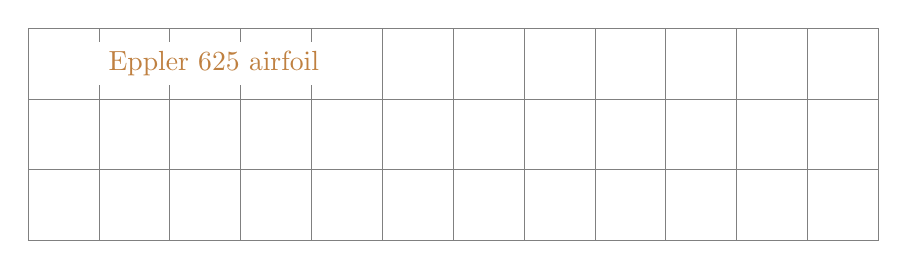
\begin{tikzpicture}[scale=0.9]
			\draw [help lines] (-1,-1) grid (11,2);
			\draw[scale=10,brown,thick] plot file{data/e625profile.dat} -- cycle;
			\node[brown,fill=white,right] at (0,1.5) {Eppler 625 airfoil};
			\end{tikzpicture}
		\caption{A plot of an Eppler 625 airfoil, to illustrate the plotting of data points from a file, data from \textcite{airfoils}}\label{fig:airfoil}
	\end{figure}
\end{frame}

\section{Plotting analytical functions}
It's also easy to plot functions in axes as shown in \cref{fig:analyticalfunctions}. In this example, three analytical functions are plotted. Inspect the source code to verify that these functions are analytically given.

\begin{figure}[htbp]\centering
    \def\funA{4*x*x-20*x-50} % definition of function A
    %\def\a{4}\def\b{-20}\def\c{-50}
        \begin{tikzpicture}
            \begin{axis}[
                    xmin=-6.28,xmax=6.28,
                    samples=200,
                    legend pos= outer north east,
                    legend cell align=left,
                    ]
                  \addplot[blue,ultra thin](x,{\funA}); % braces needed to protect
                  \addlegendentry{$y=4x^2-20x-50$};
                  \addplot[red,dashed](x,{100*sin(x*180/3.14)}); % braces needed to protect
                  \addlegendentry{$y=100\sin x$};
                  \addplot[olive, thick]({0.2*x*x*x},-40*x); % braces needed to protect
                  \addlegendentry{$x=f(y) \rightarrow$ see source code};
            \end{axis}
        \end{tikzpicture}
	\caption{Example of the plotting of some analytical functions}\label{fig:analyticalfunctions}
\end{figure}

\section{Plotting experimental data against a model}
It is also possible to plot data points together with an analytical model. This is shown in \cref{fig:psat} where experimental data is plotted against an parabolic model.

\begin{figure}[htbp]\centering
	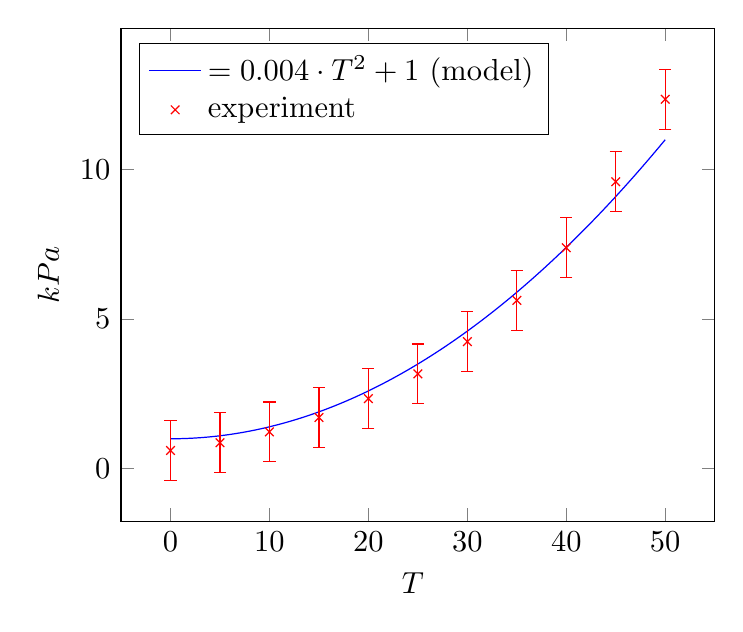
\begin{tikzpicture}[scale=1.1]
		\begin{axis} [
		xlabel=$T\ \unitschart{\si{\celsius}}$,
		ylabel= $\psat\unitschart{kPa}$,
		ylabel near ticks,
		legend pos= north west,
		legend cell align=left,
		]
		\addplot[blue,domain=0:50,samples=100]{0.004*x^2+1};
        \addlegendentry{$\psat=0.004\cdot T^2+1$ (model)}
		\addplot[red,only marks, mark=x,error bars/y dir =both,error bars/y fixed = 1] coordinates {
			(0,0.61) (5,0.87) (10,1.23) (15,1.71) (20,2.34) (25,3.17) (30,4.25) (35,5.6286) (40,7.39) (45,9.5944) (50,12.352)};
			\addlegendentry{experiment};
		\end{axis}
	\end{tikzpicture}
	\caption{Example of a plot of an analytical model against experimental data with error bars; here: the saturation pressure of water as function of temperature}\label{fig:psat}
\end{figure}

\section{Predefining plot settings}
It's also possible to predefine the settings of charts. See for instance the definition of \verb|axespsychro| in the style file \verb|myDrawingStuff.sty| and how it is used as an option in: \verb|\begin{axis}[axespsychro]| in the source code of \cref{fig:psychrochart} and \cref{fig:psychrochart2}. Both charts have exactly the same appearance because of the same predefined settings.

\begin{figure}[ht]\centering
		\begin{tikzpicture}[scale=1]
    		\begin{axis}[axespsychro]
        		\drawsaturationline{sat};
        		\coordinate (A) at (axis cs: 30,10);
        		\coordinate (B) at (axis cs: 19.2,14.3);
        		\coordinate (C) at (axis cs: 13.5,10);
        		\draw [process,deco=0.6] (A) -- (B) node [above left] {$T_\up{WB}$};  
        		\draw [process,deco=0.6] (A) -- (C) node [above left] {$T_\up{DP}$}; 
        		\draw [helpline] (A) -- (axis cs:30,0) node [above right] {$T_\up{DB}$}; 
        		\draw [helpline] (A) -- (axis cs:50,10); % 
        		\drawdot{A};\drawdot{B};\drawdot{C};
    		\end{axis}
		\end{tikzpicture}
		\caption{Example of a simplified psychrometric chart with predefined settings; here: indication of the dew point and the wet bulb temperature}\label{fig:psychrochart}
\end{figure}

\begin{figure}[ht]\centering
		\begin{tikzpicture}[scale=1]
			\begin{axis}[axespsychro]
				\drawsaturationline{sat};
				\coordinate (A) at (axis cs: 40,5);
                \coordinate (B) at (axis cs: 4.5,5);
				\draw [process,deco=0.5] (A) -- (B) node [above left] {$T_\up{DP}$}; % 
				\draw [helpline] (A) -- (axis cs: 40,0); % 
				\draw [helpline] (A) -- (axis cs: 50,5); % 
				\drawdot{A};\drawdot{B};
				%\tekenisoHlijnenoppsychrokaart; % teken isenthalpen
			\end{axis}
		\end{tikzpicture}
		\caption{Example of a second psychrometric chart with the same predefined settings; here: indication of the dew point}\label{fig:psychrochart2}
\end{figure}

\section{Grouping of plots}
Plots can be grouped in such a way that they share the same axes, see example in \cref{fig:groupplot}.

\begin{frame}{An example of a group plot with shared axes}
	\begin{figure}[ht]\centering
		\input{figs/groupplot} % if the code for a drawing is long, you can opt to put it in a separate file
		\caption{The axes can be shared in group plots, here: impact of surface area on heat exchanger performance}\label{fig:groupplot}
	\end{figure}
\end{frame}

\section{Plotting data from an external file}
Data can also be read from external files and then plotted, as in \cref{fig:thermalpower}. Even if the data in the file contains date- and timestamp (like for instance of the type \texttt{YYYY-MM-DD HH:MM}) they can still be plotted by using the TikZ-library \texttt{dateplot}. An example of such a plot is shown in \cref{fig:weatherdata}. The meteo data was fetched from \href{https://mesonet.agron.iastate.edu/request/download.phtml?}{Iowa Environmental Mesonet (IEM)} from Iowa State University. The IEM maintains an ever growing archive of automated airport weather observations from around the world.

\begin{frame}{Example of plotting data from a file}
    \begin{figure}[ht]\centering
        \begin{tikzpicture}[scale=0.8]
          \begin{axis}[
              width=0.9\linewidth, % Scale the plot to \linewidth
              grid=major, 
              grid style={dashed,gray!30},
              xlabel={Time}, % Set the labels
              ylabel={Thermal power},
              x unit=\si{\hour}, % Set the respective units
              y unit=\si{\kilo\watt}, % Set the respective units
              legend pos= north east,
              ]
              \addplot[cyan,mark=x] table[x index=0, y index=1,col sep=comma] {data/data_heat.csv}; % read data from file
              \legend{building H}
          \end{axis}
        \end{tikzpicture}
        \caption{Example of plotted data read from an external csv-file; here: thermal power demand from a building during one week}\label{fig:thermalpower}
    \end{figure}
\end{frame}

\begin{frame}{Example of plotting data with dates from a file}
    \begin{figure}[ht]\centering
        \begin{tikzpicture}[scale=0.9]
              \begin{axis}[
                width=0.8\linewidth,
                date coordinates in=x, % to indicate that the dates are in x-axis
                %xmin=2020-03-01 00:00,
                %xmax=2020-03-07 23:59,
                xtick distance=1, % set `xtick distance' to 24 hours (24/24)
                % xtick=data, % to use every entry as xtick
                xticklabel={\day-\month},
		        xlabel={Temperature data for Brookneal Virginia (USA), first week of April '20},
                ylabel={Temperature},
                y unit=\si{\celsius}, % Set the respective units
                legend pos=south east, % to place the legend
                legend cell align=left, % to align the text in the legend
                ]
                \addplot [red] table [col sep=comma,x index=1, y index=2] {data/weatherVirginia.csv};
                \addplot [blue] table [col sep=comma,x index=1, y index=3] {data/weatherVirginia.csv};
                \legend{dry bulb temperature, dewpoint}
              \end{axis}
        \end{tikzpicture}
        \caption{Example of data with date- and timestamps plotted with the TikZ-library \texttt{dateplot}; here: some weather data during one week}\label{fig:weatherdata}
    \end{figure}
\end{frame}

\mode<all> 
% Required because of the \mode* command at the beginning of this file.
% See beameruserfile.pdf section 21.3 for more info % examples of plots and drawings
		%\include{appendices/mathsymbols} % often-used math-symbols
		%\chapterOrPart{Greek symbols}\label{ch:greeksymbols}

\begin{table}[ht!]\centering\small
\caption{Greek symbols in \LaTeX}\label{tab:greeksymbols}
    \begin{tabular}{cl|cl}
        \toprule
        lowercase symbol	    &	\LaTeX  	     &	uppercase symbol	  &	 \LaTeX\\[+2ex]	
        $\alpha$	&	\verb|\alpha|	 &   &	\\
        $\beta$	    &	\verb|\beta|	 &   &	\\
        $\gamma$	&	\verb|\gamma|	 & $\Gamma$	&	\verb|\Gamma|	\\
        $\delta$	&	\verb|\delta|	 &  $\Delta$	&	\verb|\Delta|	\\
        $\epsilon$	&	\verb|\epsilon|	 &   &	\\
        $\zeta$	    &	\verb|\zeta|	 &   &	\\
        $\eta$	    &	\verb|\eta|	 &   &	\\
        $\theta$	&	\verb|\theta|	 &   $\Theta$	&	\verb|\Theta|	\\
        $\iota$	    &	\verb|\iota|	 &   &	\\
        $\kappa$	&	\verb|\kappa|	 &   &	\\
        $\lambda$	&	\verb|\lambda|	 &      $\Lambda$	&	\verb|\Lambda|	\\
        $\mu$	&	\verb|\mu|	 &   &	\\
        $\nu$	&	\verb|\nu|	 &   &	\\
        $\xi$	&	\verb|\xi|	 &    $\Xi$	&	\verb|\Xi|	\\
        $\pi$	&	\verb|\pi|	 &    $\Pi$	&	\verb|\Pi|	\\
        $\rho$	&	\verb|\rho|	 &   &	\\
        $\sigma$	&	\verb|\sigma|	 &   $\Sigma$	&	\verb|\Sigma|	\\
        $\tau$	&	\verb|\tau|	 &   &	\\
        $\upsilon$	&	\verb|\upsilon|	 &    $\Upsilon$	&	\verb|\Upsilon|	\\
        $\phi$	&	\verb|\phi|	 &   $\Phi$	&	\verb|\Phi|		\\
        $\chi$	&	\verb|\chi|	 &   &	\\
        $\psi$	&	\verb|\psi|	 &    $\Psi$	&	\verb|\Psi|		\\
        $\omega$	&	\verb|\omega|	 &    $\Omega$	&	\verb|\Omega|	\\
        \bottomrule
    \end{tabular}
\end{table}

\mode<all> % Greek symbols
		%\include{appendices/isa} % example of a table in appendix
		
	\backmatter % arabic page numbers & chapters not numbered
	    \nocite{*} % uncomment to include all bib file entries in bibliography
		\printbibliography\label{sec:bibliography}
		%\listoftodos
\end{document}

% Here you can put whatever you want, for instance a to do list. It will never be seen and compiled by LaTeX.
